\documentclass[11pt]{article}
\usepackage[T1]{fontenc}
\usepackage[utf8]{inputenc}
\usepackage{lmodern}
\usepackage{graphicx} % Required for inserting images
\usepackage{float}
\usepackage[margin=2.5cm]{geometry}
\usepackage{amsmath}
\usepackage{amssymb}
\setlength{\parindent}{0pt}
\setlength{\parskip}{0.6em}
\setlength{\abovedisplayskip}{6pt}
\setlength{\belowdisplayskip}{6pt}
\setlength{\abovedisplayshortskip}{0pt}
\setlength{\belowdisplayshortskip}{4pt}
\usepackage{xcolor}
\usepackage[colorlinks=true,
            linkcolor=black,
            citecolor=blue!60!black,
            urlcolor=blue!60!black]{hyperref}
\usepackage{amsthm}
\usepackage[numbers,sort&compress]{natbib}
\newtheorem{theorem}{Theorem}
\newtheorem{definition}{Definition}
\theoremstyle{remark}
\newtheorem*{remark}{Remark}
\theoremstyle{plain}
\allowdisplaybreaks

\begin{document}

% ============================================================
% GAI Declaration
% ============================================================
\thispagestyle{empty}

\noindent{\Large\bfseries Deklaration for brug af GAI-værktøjer}

\bigskip
\noindent\fbox{%
\begin{minipage}{\dimexpr\textwidth-2\fboxsep-2\fboxrule\relax}
\smallskip

\noindent\fbox{%
\begin{minipage}{\dimexpr\linewidth-2\fboxsep-2\fboxrule\relax}
\smallskip

\noindent$\boxtimes$\enspace\textbf{Jeg/vi har benyttet generativ kunstig intelligens til udfærdigelse af dette projekt}
\textit{(sæt kryds). Oplist, hvilke GAI-værktøjer der er benyttet (husk version):}
\begin{itemize}
  \item Claude sonnet 4.6
\end{itemize}

\vspace{5em}
\smallskip
\end{minipage}}

\medskip
\noindent\textbf{Jeg/vi har brugt GAI-værktøjer på følgende vis:}
\begin{itemize}
  \item latex kode hjælp både debugging, hjælp til at bygge lidt mere spøjse objekter såsom denne side og overordnet struktur af latexcode
  \item Debugging af python kode
  \item korrekturlæsning
\end{itemize}


\medskip


\medskip
\noindent\textit{For hvert relevant område forklares, hvordan GAI er benyttet (se forklaringer af de
forskellige anvendelsesmuligheder på \href{https://studypedia.au.dk}{Studypedia}). Beskriv
f.eks.\ kortfattet, hvordan informationen blev genereret, og forklar, hvordan outputtet er
anvendt i din/jeres opgave.}

\smallskip
\end{minipage}}

\newpage

\begin{titlepage}
  \centering
  \vspace*{3cm}

  {\large Bachelor's Project}\\[2cm]

  {\LARGE\bfseries  Lewis Style Fourier-Pricing and the Heston model\\[0.4em]}
  {\large\itshape Lewis-inspireret Fourier-prissætning og Heston modellen}\\[3cm]

  \begin{tabular}{rl}
    \textbf{Supervisor:}    & Elisa Nicolato \\[0.4em]
    \textbf{Date:}          & [submission date] \\
  \end{tabular}

  \vfill
\end{titlepage}
\newpage
\section*{Abstract}
The Black--Scholes--Merton model prices options under the assumption of constant volatility, which implies a flat implied volatility surface. In practice this is not the case, and any serious attempt needs to account for the smile and structure observed in the market.

This paper covers the full pipeline of the Heston model, from theory through to calibration on real market data. Starting from the Lewis \cite{lewis2001}  Fourier pricing framework, we derive a general formula for pricing a covered call given any characteristic function satisfying mild regularity conditions, and then derive the Heston characteristic function from the Feynman--Kac equations, verifying that it meets those conditions. On the implementation side we run an experiment comparing different quadrature choices and the impact of an analytical gradient due to Germano et al.\cite{germano2017} on calibration speed. Finally, we calibrate the model to S\&P 500 closing option prices from 13 November 2019 under two different weighting schemes and examine how the choice of objective function shapes the fitted implied volatility surface.

\newpage
\section*{Resumé}
Black-Scholes-Merton modellen prisfastsætter optioner under antagelsen om konstant volatilitet, som medfører en flad volatility-surface. Dette er dog langt fra hvad der observeres i praksis og et særiøst forsøg på at modellere optionspriser 
blivder derved nød til at tage højde for volatilitets-smilet og dens opførsel når vi går længere ud på kurven.

Denne opgave dækker hele processen af prisfastsættelse på Heston modellen, fra Fourier-teori til model kalibrering. Med udgangspunkt i Lewis \cite{lewis2001} Fourier-metoder, 
klæder vi os på til at prisfastsætte et Covered Call på en generel karakteristisk funktion, under nogle regularitetsbetingelser. Vi udleder herefter Heston-modellens karakteristiske funktion ud fra Feynman-kac betingelserne og verificerer at fourier metoderne kan bruges. 
på implementeringssiden kører vi et eksperiment der sammenligner hastigheden af kalibrering udført med forskellige kvadraturer, samt brug af en analytisk gradient fra Germano et al.\cite{germano2017}. Til slut kalibrer vi modellen til lukkepriser på S\&P 500 indeks optioner fra 13/11/2019 under to forskellige vægtningsmetoder og undersøger hvordan den ændrede objektivfunktion påvirker den tilpassede volatility-surface

\newpage
\tableofcontents
\label{sec:toc}
\newcommand{\sectionwithtoclink}[1]{\section[#1]{\texorpdfstring{\hyperref[sec:toc]{#1}}{#1}}}

\let\origsubsection\subsection
\renewcommand{\subsection}[1]{\origsubsection[#1]{\texorpdfstring{\hyperref[sec:toc]{#1}}{#1}}}
\let\origsubsubsection\subsubsection
\renewcommand{\subsubsection}[1]{\origsubsubsection[#1]{\texorpdfstring{\hyperref[sec:toc]{#1}}{#1}}}

\sectionwithtoclink{Introduction}

The Black--Scholes--Merton (BSM) model prices options under the assumption of constant volatility across strikes and maturities.
This implies a flat implied volatility surface which, in practice, is far from the case. Market-implied volatilities are both skewed and far from
constant across maturities, so any serious attempt to model option prices must therefore account for stochastic volatility.

The Heston model~\cite{heston1993} is one such model, extending BSM by letting the volatility follow a mean-reverting square-root (CIR) process
which is allowed to be correlated with the asset. One of the advantages of the Heston model is that it captures a lot of the shape of the volatility surface,
while still having a nice analytical expression for the characteristic function of the log asset price. The CF being well enough behaved turns out to be all one needs to price derivatives
due to Fourier methods, which we will use the beginning of this paper to show how.

This paper tries to develop as much of the pipeline as possible. After finding a pricing formula for calls when the CF has certain properties,
we spend some time deriving the original expression for the Heston CF and verify that it has the aforementioned properties. Moving on to implementation, we set
up an experiment to compare quadratures as well as the impact of introducing an analytical gradient~\cite{germano2017} on the speed of calibration. Finally,
we calibrate the model to S\&P 500 closing option prices under two weighting schemes and examine how the choice of objective function shapes the fitted implied volatility surface.



Notation Note: We take a lot of expectations in the beginning of the paper, usually of what turns out to be stochastic processes when taking these we know their values at time 0 making every expectation $\mathbb{E}_{(x_0,v_0)}$ 
instead of writing this every time we will simply define this as the default probabilitymeasure. Usually we like to note information up to a time as $\mathcal{F}_t$ in this paper i've choosen to drop the filters i.e work from the filter $\mathcal{F}_0$. One should 
note that since the heston model is a markov process everything still works as every expectation is essentially $\mathbb{E}_{(x_0,v_0)}$ and by the markov property 
$\mathbb{E}_\mu[f(X_{t+s},V_{t+s})|\mathcal{F}]=\mathbb{E}_{(x_t,v_t)}[f(X_s,V_s)]$ for $f$ non negative and measuerable, so this actually dosen't change anything simply set $T=T-t\quad x_0=x_t,v_0=v_t$





\sectionwithtoclink{Fourier Pricing}

When dealing with more complex models for asset prices than the Black--Scholes model, the fact that there is no known analytical
density for the underlying at time $T$ becomes a common problem, as for a european derivative the calculation $\mathbb{E}[w(S_T)]$ is
no longer a straightforward integration exercise. For a subset of these more complicated models we've discovered analytical
expressions for their characteristic functions. Using these as the means to price derivatives is exactly the task we will address over the next section.

\subsection{The Lewis Formula}
The following result is due to Lewis~\cite{lewis2001}.
Let $X_t$ be a process with the ``flipped'' characteristic function $u\to\psi(-u)$, assume that this function is analytic and regular on the strip $\mathcal{S}_{-\psi}$.
Let $w(x)\geq0$ with generalised Fourier transform $\hat{w}$ on strip of regularity $\mathcal{S}_w$. For
$\alpha\in \{v\in\mathbb{R} : \{x+i v:x\in\mathbb{R}\}\subseteq \mathcal{S}_M=\mathcal{S}_{-\psi} \cap \mathcal{S}_w\}=A$
\begin{align}
\mathbb{E}[w(X_T)] = \frac{1}{2\pi}\int_{-\infty+i\alpha}^{\infty+i\alpha}\psi(-z)\hat{w}(z) dz
\end{align}
\begin{proof}
Assume that $A$ is non-empty.
Let $\alpha\in A$.
By the inversion theorem and the choice of $\alpha$:
\begin{align}
\mathbb{E}[w(X_T)]&=\int_{-\infty}^{\infty}w(x)\frac{1}{2\pi}\int_{-\infty+i\alpha}^{\infty+i\alpha}\exp(-izx)\psi(-z) dzdx
\end{align}
We check that the product is integrable via Tonelli's theorem:
\begin{equation}\int_{-\infty}^{\infty} \int_{-\infty}^{\infty}
|w(x)| \cdot e^{-\alpha x} \cdot |\psi(-(u+i\alpha))|\, du\, dx < \infty\end{equation}
since $w(x)\exp(-\alpha x)\in L^1$ and $\psi(-(u+i\alpha))\in L^1$
since $\alpha\in A$, the integral is finite.
Thus we may apply Fubini's theorem:
\begin{align}
(3)&=\int_{-\infty+i\alpha}^{\infty+i\alpha}\psi(-z)\frac{1}{2\pi}\int_{-\infty}^{\infty}\exp(-izx)w(x) dxdz \\
&=\frac{1}{2\pi}\int_{-\infty+i\alpha}^{\infty+i\alpha}\psi(-z)\hat{w}(z) dz\quad
\end{align}
\end{proof}
Now, turning this into something useful for finance, we can pick a model of our choice with a nice characteristic function, a positive payoff function, and then calculate this integral.

\subsection{Pricing Options via the Covered Call/Cash Secured Put}
Throughout this section we work at time $t=0$ with maturity $T$, pricing today's option price.
When one wants to apply this method to pricing options directly, it turns out that the available set $\mathcal{S}_M$ will narrow and widen depending
on one's choice of parameters, which will make the whole task of calibrating a volatility surface based on a model more difficult.
To circumvent this problem we will not price a call directly but rather price a covered-call.\\
A covered call is what one gets by buying a forward on the underlying and selling a call on it, ``covering'' one's downside, giving the following payoff at time $T$:
\begin{align}
e^{X_T}-\max(0,e^{X_T}-K)=\min(e^{X_T},K) \\
Z = e^{-rT}\mathbb{E}^{\mathbb{Q}}[\min(e^{X_T},K)]
\end{align}
then creating the call by replication.
\begin{equation}C = e^{-rT}F_T-Z
\end{equation}
noting that by put-call parity
\begin{equation}P = C-e^{-rT}F +e^{-rT}K = e^{-rT}K-Z
\end{equation}
so let's find the strip of regularity for this payoff
\begin{align}
    z= \beta+i \alpha \in S_f \Leftrightarrow \int_{-\infty}^{\infty}e^{-\alpha x}|\min(e^{x},K)|dx<\infty\\
\int_{-\infty}^{\infty}e^{-\alpha x}|\min(e^{x},K)|dx = \int_{-\infty}^{\log(K)}e^{(1-\alpha) x} dx+\int_{\log(K)}^{\infty}e^{-\alpha x}K dx
\end{align}
Both integrals are positive, we simply need to figure out when they are finite, we do this rather simply with monotone convergence:

\textbf{First integral:}\\
For $\alpha =1$ we clearly diverge.\\
For $\alpha \neq 1$:
\begin{equation}\int_{-\infty}^{\log(K)}e^{(1-\alpha) x} dx= \lim_{n\to \infty}[-\frac{e^{(1-\alpha) x}}{1-\alpha}]^{\log(K)}_{-n}<\infty \Leftrightarrow \alpha<1
\end{equation}

\textbf{Second integral:}\\
For $\alpha=0$ it explodes.\\
For $\alpha\neq 0$:
\begin{align}
\int_{\log(K)}^{\infty}e^{-\alpha x}K dx = \lim_{n\to \infty}[-\frac{e^{-\alpha x}}{\alpha}]_{\log(K)}^n<\infty \Leftrightarrow \alpha>0
\end{align}
Combining these results,
\begin{equation}z= \beta+i \alpha \in S_f \Leftrightarrow \alpha \in (0,1)
\end{equation}
Now let's calculate the generalised Fourier transform when it exists.
Let $\alpha \in (0,1)$:
\begin{align}
    \hat{w} (\beta+i \alpha)&=\int_{-\infty}^{\infty}e^{i(\beta+i \alpha)x}w(x) dx\\
    &=\int_{-\infty}^{\log(K)}e^{i(\beta+i \alpha)x}e^x dx + \int_{\log(K)}^{\infty}e^{i(\beta+i \alpha)x}K dx\\
    &=\int_{-\infty}^{\log(K)}e^{i(\beta+i (\alpha-1))x} dx + \int_{\log(K)}^{\infty}e^{i(\beta+i \alpha)x}K dx\\
    &= \lim_{n\to \infty}[\frac{e^{i(\beta+i (\alpha-1))x}}{i(\beta+i (\alpha-1))}]^{\log(K)}_{-n}+K \lim_{n\to \infty}[\frac{e^{i(\beta+i \alpha)x}}{i(\beta+i \alpha)}]^{n}_{\log(K)}\\
    &= \frac{e^{i(\beta+i (\alpha-1))\log(K)}}{i(\beta+i (\alpha-1))} -K \frac{e^{i(\beta+i \alpha)\log(K)}}{i(\beta+i \alpha)}\\
    &= K^{ 1+i(\beta+i \alpha)}(\frac{1}{1+i(\beta+i \alpha)} -\frac{1}{i(\beta+i \alpha)})\\
    &=\frac{K^{1+iz}}{z^2-iz}
\end{align}
where a dominated convergence argument is used on the step from line 17 to line 18, and we swap to $z=\beta+i\alpha$ on the last step.

\subsection{Existence Strip of the CF}

Consider now a storable asset $S_T$ under the risk-neutral measure $\mathbb{Q}$ in a world with constant short rate $r>0$ and continuously paid dividend $q\geq0$. Let
$X_T=\log(S_T)$, a consequence of the risk-neutral measure construction is that $\mathbb{E}[S_T]=\exp((r-q)T)S_0$.
Before moving on we want to show that the CF for basically any type of model is well defined on $\Im(u)\in(0,1)$.\\
In the following everything is happening under $\mathbb{Q}$.\\
Let $u=\beta + i \alpha$.

for $\alpha =0$
\begin{align}
\mathbb{E}[|\exp(-iuX_T)|]=1<\infty
\end{align}

for $\alpha = 1$
\begin{align}
\mathbb{E}[|\exp(-iuX_T)|]&=\mathbb{E}[|\exp(-i(\beta+i\alpha)X_T)|]\\
&=\mathbb{E}[\exp(\alpha X_T)]\\
&=\mathbb{E}[\exp(X_T)]\\
&=\mathbb{E}[S_T]=\exp((r-q)T)S_0<\infty
\end{align}
for $\alpha\in (0,1)$, notice that $x\to x^\alpha$ is concave, then by Jensen's inequality
\begin{align}
\mathbb{E}[\exp(\alpha X_T)]&=\mathbb{E}[(\exp(X_T))^\alpha ]\\
\leq (\mathbb{E}[\exp(X_T)])^\alpha &= S_0^\alpha  \exp(\alpha (r-q)T)<\infty\\
&\Rightarrow \{z\in \mathbb{C} : \operatorname{Im}(z)\in[0,1]\}
\end{align}



\subsection{A General Formula for a Covered-Call Price Using Lewis}
For log-asset dynamics $X_T=\log(S_T)$ under the risk-neutral measure $\mathbb{Q}$,
now assume that
$\{\alpha +\frac{i}{2} : \alpha\in\mathbb{R}\}\subseteq \mathcal{S}_{-\psi} \cap \mathcal{S}_w$. Choosing to integrate along the line $\{\alpha +\frac{i}{2} : \alpha\in\mathbb{R}\}$ we get a simple formula for the covered call at $t=0$.

\begin{theorem}[Covered-Call price]
Consider the covered call payoff function $w(x)=\min(e^x,K)$ and log-asset dynamics $X_T=\log(S_T)$ under $\mathbb{Q}$. Then the covered call price at $t=0$ is:
\begin{equation}Z =\frac{e^{\frac{k}{2}-rT}}{\pi}\int_{0}^{\infty}\frac{\operatorname{Re}[\psi(u-\frac{i}{2})e^{-i k u}]}{u^2+\frac{1}{4}}du
\end{equation}
where $k=\log(K)$ and $\psi$ is the extended characteristic function of $X_T$
\end{theorem}
\begin{proof}
By assumption $\{\alpha +\frac{i}{2} : \alpha\in\mathbb{R}\}\subseteq \mathcal{S}_{-\psi} \cap \mathcal{S}_w$.
We choose to integrate across the line $\{\alpha +\frac{i}{2} : \alpha\in\mathbb{R}\}$, i.e.\ pick $\alpha =1/2$ in the Lewis formula. Taking the expression for $\hat{w}$ that we found:
\begin{align}
    \mathbb{E}[\min(e^{X_T},K)]&=\frac{1}{2\pi}\int_{-\infty+i\alpha}^{\infty+i\alpha}\psi(-z)\hat{w}(z) dz\quad\\
    &=\frac{1}{2\pi}\int_{-\infty+i\alpha}^{\infty+i\alpha}\psi(-z)\frac{K^{1+iz}}{z^2-iz}dz \quad\\
    &=\frac{1}{2\pi}\int_{-\infty+i\alpha}^{\infty+i\alpha}\mathbb{E}[e^{-izX_T}]\frac{K^{1+iz}}{z^2-iz}dz\\
    &=\frac{K}{2\pi}\int_{-\infty+i\alpha}^{\infty+i\alpha}\mathbb{E}[e^{-izX_T}]\frac{K^{iz}}{z^2-iz}dz
\end{align}
now we change variable to $u=z-i\alpha$, note:
\begin{align}
(u+\frac{i}{2})^2-i(u+\frac{i}{2})&=u^2+iu-\frac{1}{4} -iu+\frac{1}{2}\\
&=u^2+\frac{1}{4}\\
\frac{K}{2\pi}\int_{-\infty+i\alpha}^{\infty+i\alpha}\mathbb{E}[e^{-izX_T}]\frac{K^{iz}}{z^2-iz}dz
&=\frac{K}{2\pi}\int_{-\infty}^{\infty}\mathbb{E}[e^{-iuX_T}e^{\frac{X_T}{2}}]\frac{K^{iu}K^{-\frac{1}{2}}}{u^2+\frac{1}{4}}du\\
&=\frac{K^{\frac{1}{2}}}{2\pi}\int_{-\infty}^{\infty}\mathbb{E}[e^{-iuX_T}e^{\frac{X_T}{2}}]\frac{K^{iu}}{u^2+\frac{1}{4}}du
\end{align}
setting $k = \log(K)$
\begin{align}
    &=\frac{e^{\frac{k}{2}}}{2\pi}\int_{-\infty}^{\infty}\psi(-u-\frac{i}{2})\frac{e^{i k u}}{u^2+\frac{1}{4}}du
\end{align}
now we notice:
\begin{align}
    \overline{\psi(-u-\frac{i}{2})}&=\overline{\mathbb{E}[e^{-iuX_T}e^{\frac{X_T}{2}}]}\\
    &=\mathbb{E}[\overline{e^{-iuX_T}e^{\frac{X_T}{2}}}]\\
    &=\mathbb{E}[e^{iuX_T}e^{\frac{X_T}{2}}]\\
    &=\psi(u-\frac{i}{2})\\
    \overline{e^{iku}}&=e^{-iku}\\
    \overline{\frac{1}{u^2+\frac{1}{4}}}&=\frac{1}{(-u)^2+\frac{1}{4}}
\end{align}
combining with the result,
\begin{align}
f\in L^1 \overline{f(x)}=f(-x)\Rightarrow \int_{-\infty}^{\infty}f(x)dx = 2\int_{0}^{\infty}\operatorname{Re}[f(x)]dx=2\int_{0}^{\infty}\operatorname{Re}[f(-x)]dx
\end{align}
we then have
\begin{align}
    \frac{e^{\frac{k}{2}}}{2\pi}\int_{-\infty}^{\infty}\psi(-u-\frac{i}{2})\frac{e^{i k u}}{u^2+\frac{1}{4}}du
    &=\frac{e^{\frac{k}{2}}}{\pi}\int_{0}^{\infty}\frac{\operatorname{Re}[\psi(u-\frac{i}{2})e^{-i k u}]}{u^2+\frac{1}{4}}du
\end{align}
Discounting then gives
\begin{equation}
Z = e^{-rT}\mathbb{E}[\min(e^{X_T},K)] = \frac{e^{\frac{k}{2}-rT}}{\pi}\int_{0}^{\infty}\frac{\operatorname{Re}[\psi(u-\frac{i}{2})e^{-i k u}]}{u^2+\frac{1}{4}}du
\end{equation}
\end{proof}
\begin{remark}
We can now price the put and call by replication:
\begin{align}
C &= e^{-rT}F_T-Z = e^{-rT}F_T-\frac{e^{\frac{k}{2}-rT}}{\pi}\int_{0}^{\infty}\frac{\operatorname{Re}[\psi(u-\frac{i}{2})e^{-i k u}]}{u^2+\frac{1}{4}}du\\
P &= Ke^{-rT}-\frac{e^{\frac{k}{2}-rT}}{\pi}\int_{0}^{\infty}\frac{\operatorname{Re}[\psi(u-\frac{i}{2})e^{-i k u}]}{u^2+\frac{1}{4}}du
\end{align}
\end{remark}

\sectionwithtoclink{The Heston Model}



\subsection{The Model}
The Heston model is defined by the following stochastic differential equations (SDEs)
\begin{align}
dS_t &= (r-q)\, S_t\,dt + \sqrt{v_t}\,S_t\,dW_t^{(1)}, \\
dv_t &= \kappa(\theta - v_t)\,dt + \sigma \sqrt{v_t}\,dW_t^{(2)} \\
\rho\,dt &= dW_t^{(1)} dW_t^{(2)}
\end{align}
where $r\geq 0$ is the constant risk-free rate, $q\geq0$ is a continuously paid dividend yield,
 $\kappa>0$ is the mean reversion factor,
 $\theta>0$ is the long-run variance,
 $\sigma>0$ is the so called vol-of-vol and
 $\rho\in[-1,1]$ is the correlation between the two Brownian motions driving the model,
 and $2\kappa\theta > \sigma^2$ which is called the Feller condition, forcing the variance process to be positive almost surely.




Applying It\^{o}'s lemma with $X_t=\log(S_t)$,
we get an equivalent model description
\begin{align}
dX_t &= \left(r -q- \frac{1}{2} v_t\right) dt + \sqrt{v_t}\, dW_t^{(1)}\\
dv_t &= \kappa(\theta - v_t)\,dt + \sigma \sqrt{v_t}\,dW_t^{(2)} \\
\rho\,dt &= dW_t^{(1)} dW_t^{(2)}
\end{align}
The neat thing about this extension is letting practitioners capture some of the behaviour they observe in real markets in their models,
namely letting the volatility process be stochastic and correlated with the underlying, also roughly letting the long-term vol converge towards
an expected level, matching the shape of the volatility surface flattening out on longer maturities. A complication with this model is the lack of an
analytical density for $X_T$, but knowing what we do about Fourier pricing we simply need the extended characteristic function to have an analytical expression,
which it turns out to do. But how does the model actually behave? To answer this question I've made some simulations using a Milstein-corrected Euler scheme as it is done
in~\cite{gatheral2006}

\begin{figure}[H]
  \centering
  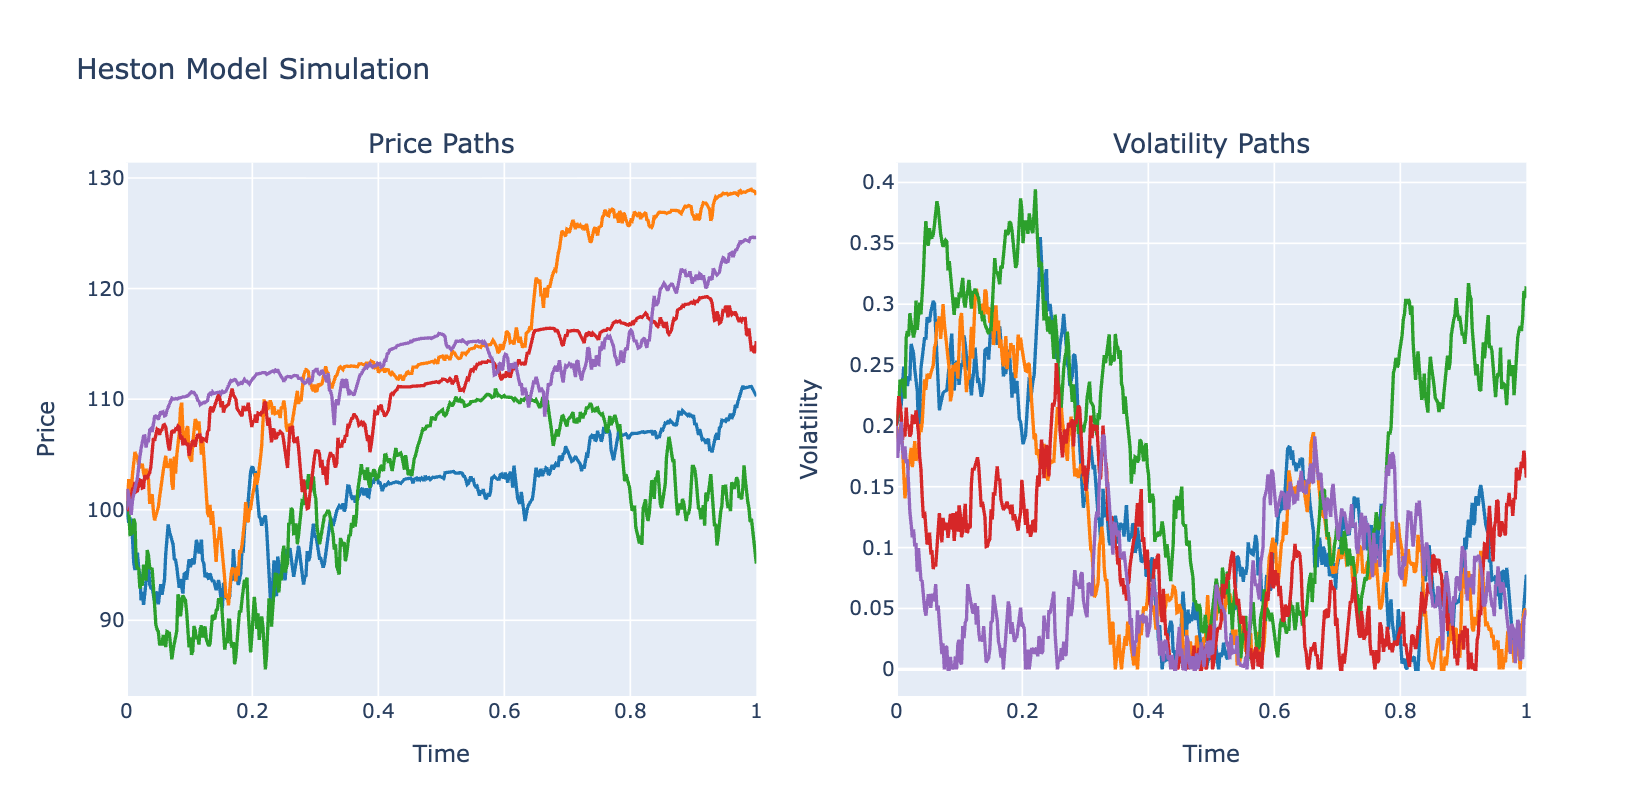
\includegraphics[width=\textwidth]{images/model_simulation.png}
  \caption{Simulated Heston model paths for the asset price and variance process using a Milstein-corrected Euler scheme ($S_0=100$, $v_0=0.04$, $\kappa=2.0$, $\theta=0.04$, $\sigma=0.6$, $\rho=-0.7$, $r=0.05$, $q=0.02$, $T=1$, $N=512$).}
  \label{fig:heston-simulation}
\end{figure}
In short, when markets go up they are more steady, but when they go down volatility spikes and we see more fluctuations.


\subsection{The Heston CF}
In this next part of the paper we will be deriving the characteristic function of the stochastic variable which solves the SDEs
which define the Heston model, we will be deriving the expression of the CF that Heston found in his original paper~\cite{heston1993},
starting from the Feynman--Kac conditions, which are essentially the same as what Heston does.
Assuming some regularity which the Heston SDEs satisfy, the Feynman--Kac formula gives us:
for every Borel function with polynomial growth f, a function $u:\mathbb{R}^+\times\mathbb{R}^n\rightarrow \mathbb{R}$ which satisfies
\begin{itemize}
\item[i)] $\frac{\partial u}{\partial t}(t, x) = Lu(t, x)\quad \forall t\geq0,x\in \mathbb{R}^n$\\
\item[ii)] $u(0, x) = f(x)\quad \forall x\in \mathbb{R}^n$\\
\item[iii)] $\exists C\in L^1_{loc}(\mathbb{R}),p\geq 0:\quad  \|\nabla u(t, x)\| \leq C(t)\left(1 + \|x\|^p\right)\quad \forall t\geq 0, x\in \mathbb{R}^n$,
\end{itemize}

satisfies
\begin{align}
\Rightarrow \mathbb{E}[f(X_t)] &=u(t,x)\quad\forall t\geq0,x\in \mathbb{R}^n
\end{align}

The idea of the proof is to use Feynman--Kac to get the characteristic function by setting $f(x,v)=e^{i\phi x}$ and guessing the solution
$u(t,x,v)$ for every $\phi\in\mathbb{R}$, and then extending it to the strip $\{b\in\mathbb{C}:\Im(b)\in[-1,0]\}$, thus getting the slightly extended characteristic function for the model.

\begin{theorem}[Heston Characteristic Function]
The characteristic function of $X_T = \log S_T$ under the Heston model is
\begin{equation}
\psi_T(\phi) = \exp\!\bigl(C(T,\phi) + D(T,\phi)\,v_0 + i\phi\,x_0\bigr), \quad \phi\in\mathbb{R},
\end{equation}
where $x_0 = \log S_0$. The auxiliary quantities are
\begin{align}
\xi &= \sigma\rho\,i\phi - \kappa, \\
d &= \sqrt{\xi^2 + \sigma^2(\phi^2+i\phi)}, \quad \Re(d)\geq 0,\\
g &= \frac{\xi-d}{\xi+d},\qquad D_1 = \frac{-\xi+d}{\sigma^2},
\end{align}
and the coefficient functions are
\begin{align}
D(T,\phi) &= D_1\,\frac{1-e^{dT}}{1-g\,e^{dT}}, \\[6pt]
C(T,\phi) &= (r-q)\,i\phi\,T
  + \kappa\theta\,D_1\!\left[T + \frac{1-g}{dg}
    \log\!\!\left(\frac{1-g\,e^{dT}}{1-g}\right)\right].
\end{align}
\end{theorem}

Let's start off by writing up the Feynman--Kac conditions within the model:

\begin{itemize}
\item[i)]
$\frac{\partial u}{\partial t} = \left(r-q-\frac{v}{2}\right)\frac{\partial u}{\partial x}
  +\kappa(\theta-v)\frac{\partial u}{\partial v}
  +\frac{v}{2}\!\left(\frac{\partial^2 u}{\partial x^2}+\sigma^2\frac{\partial^2 u}{\partial v^2}\right)
  +\sigma\rho v\frac{\partial^2 u}{\partial x\,\partial v}$
\item[ii)] $u(0, x, v) = \exp(i\phi x)$
\item[iii)] $\exists C\in L^1_{loc}(\mathbb{R}),p\geq 0:\quad  \|\nabla u(t, x, v)\| \leq C(t)\left(1 + \|(x,v)\|^p\right)\quad \forall t\geq 0, (x,v)\in \mathbb{R}^2$,
\end{itemize}
we make an affine ansatz
\begin{equation}u(t,x,v,\phi)= \exp(C(t,\phi)+D(t,\phi)v+i\phi x)\end{equation}
where we can calculate all the relevant partial derivatives
\begin{equation}
\begin{aligned}
u_x &= i\phi \,u, \\
u_v &= D\,u, \\
u_t &= (C' + D'v)\,u, \\
u_{xx} &= -\phi^2\,u, \\
u_{vv} &= D^2\,u, \\
u_{xv} &= i\phi D\,u.
\end{aligned}
\end{equation}
\begin{equation}i)\Leftrightarrow (C'+D'v)u= (r-q-\frac{1}{2}v)i\phi \,u+\kappa(\theta-v)D\,u+v\frac{1}{2}(-\phi^2\,u+\sigma^2 D^2\,u)+\sigma v\rho i\phi D\,u\end{equation}

We divide by $u$, which is non-zero (complex exponential), and combine like terms:
\begin{align}
C'+D'v = (r-q-\frac{1}{2}v)i\phi +\kappa(\theta-v)D+v\frac{1}{2}(-\phi^2+\sigma^2 D^2)+\sigma v\rho i\phi D\\
\Leftrightarrow C' + D'v=(r-q)i\phi + \kappa\theta D+v\left(-\frac{1}{2}i\phi-\kappa D+\frac{1}{2}(-\phi^2 + \sigma^2 D^2)+\sigma \rho\, i\phi D\right)
\end{align}
must be true for every v especially $v=0$ thus
\begin{align}
C' &=(r-q) i \phi+\kappa\theta D\\
D' &= \frac{1}{2}\sigma^2 D^2-\frac{1}{2}(\phi^2 + i\phi)+D(\sigma \rho\, i\phi -\kappa)
\end{align}
and similarly for ii) implies
\begin{equation}D(0)=0, \quad C(0)=0\end{equation}

The equation for $D$ is just an ODE, so let's solve it more specifically it is a Riccati equation of the form
\begin{equation}D'(t)=a(t)D(t)^2+b(t)D(t)+c(t)\end{equation}
with $a,b,c$ being constants in $t$, $f(t,D)= aD^2+bD+c \in C^\infty$ is locally Lipschitz in $D$ and a solution exists at least in some ball around $0$, which will be our $D$ from now on.\\
Let's start by finding the roots. First, define $\xi =\sigma \rho\, i\phi -\kappa$:
\begin{align}
0&= \frac{1}{2}\sigma^2 D^2-\frac{1}{2}(\phi^2 + i\phi)+D\xi\\
\Rightarrow D&=\frac{-\xi\pm d}{\sigma^2}
\end{align}
with $d=\sqrt{\xi^2+\sigma^2(\phi^2+i\phi)}$
thus by defining the roots we get
\begin{align}
D_1 &= \frac{-\xi+ d}{\sigma^2}\\
D_2 &=\frac{-\xi- d}{\sigma^2}\\
D'&=\frac{1}{2}\sigma^2(D-D_1)(D-D_2)
\end{align}
The solution to this ODE doesn't necessarily hit the roots, but we still need to note them so as not to divide by zero.\\
Here I should mention that if $0$ is a root then $D(t)=0$ solves the ODE, and by uniqueness must be the solution.

For now let's assume $D\neq D_1,D_2,\quad D_1\neq D_2,\quad D_1,D_2\neq 0$:
\begin{align}
\frac{1}{(D-D_1)(D-D_2)}&=\frac{1}{D_1-D_2}\left(\frac{1}{D-D_1}-\frac{1}{D-D_2}\right)
\end{align}
so for $D(t)\neq D_1,D_2$
\begin{align}
\frac{D'(t)}{(D(t)-D_1)(D(t)-D_2)}&=\frac{1}{D_1-D_2}\left(\frac{D'(t)}{D(t)-D_1}-\frac{D'(t)}{D(t)-D_2}\right)\\
\Rightarrow \frac{1}{2}\sigma^2&=\frac{1}{D_1-D_2}\left(\frac{D'(t)}{D(t)-D_1}-\frac{D'(t)}{D(t)-D_2}\right)
\end{align}
we remember that for u differentiable and $u(t)\neq 0$
\begin{equation}\frac{d}{dt}\log(u(t))=\frac{u'(t)}{u(t)}\end{equation}
by setting $u_1(t)=D(t)-D_1,\quad u_2(t)=D(t)-D_2$
\begin{align}
\frac{d}{dt}\log(D(t)-D_1\bigr) &=\frac{D'(t)}{D(t)-D_1}, \\
\frac{d}{dt}\log(D(t)-D_2\bigr) &=\frac{D'(t)}{D(t)-D_2}.\\
\Rightarrow\frac{d}{dt}\left[\frac{1}{D_1-D_2}\log\left(\frac{D(t)-D_1}{D(t)-D_2}\right)\right] &= \frac{1}{2}\sigma^2.\\
\Rightarrow\log\left(\frac{D(t)-D_1}{D(t)-D_2}\right)&=\frac{1}{2}\sigma^2(D_1-D_2)\,t + C\\
 D_1-D_2&=\frac{2d}{\sigma^2}\\
\Rightarrow\log\left(\frac{D(t)-D_1}{D(t)-D_2}\right)&=d t +C\\
\Leftrightarrow\frac{D(t)-D_1}{D(t)-D_2}&=\exp(dt+C)\\
\Leftrightarrow D(t)-D_1&=\exp(dt+C)(D(t)-D_2)\\
\Leftrightarrow D(t)(1-\exp(dt+C))&=D_1-D_2\exp(dt+C)\\
\Leftrightarrow D(t)&=\frac{D_1-D_2\exp(dt+C)}{1-\exp(dt+C)}
\end{align}
imposing the initial condition $D(0)=0$ and by renaming $\exp(C)=g$
\begin{align}
0=\frac{D_1-D_2g}{1-g}\Leftrightarrow g&=\dfrac{D_1}{D_2}=\frac{-\xi+d}{-\xi-d}=\frac{\xi-d}{\xi+d}\\
\Rightarrow D(t)&=D_1 \frac{1-\exp(dt)}{1-g\, \exp(dt)}
\end{align}

we should also consider if we ever have $D_1=D_2$
the short answer is no since:
\begin{align}D_1=D_2\Leftrightarrow d&=0\Leftrightarrow d^2=0\\
(\sigma \rho i \phi - \kappa)^2
&= \kappa^2 - 2\kappa \sigma \rho i \phi - \sigma^2 \rho^2 \phi^2\\
d^2&= \kappa^2 + \sigma^2(1-\rho^2)\phi^2 + i\phi(\sigma^2 - 2\kappa \sigma \rho)
\end{align}

but we assume  $\kappa>0,|\rho|\leq 1 \Rightarrow \Re (d^2)>0\Rightarrow d\neq 0$
thus we can never have $D_1=D_2$ but having a 0-root can and will happen actually
\begin{equation}D' \text{ has 0 as root}\Leftrightarrow \phi^2+i\phi=0\Leftrightarrow \phi\in \{0,-i\}\end{equation}
but $\phi\in \mathbb{R}$ thus
\begin{equation}\Leftrightarrow \phi=0\end{equation}
we've proven that when we have 2 non-zero roots that for  $D(t)\notin \{D_1,D_2\}$
\begin{equation}D(t)=D_1 \frac{1-\exp(dt)}{1-g\, \exp(dt)}\end{equation}
but does D ever hit the roots? i.e
\begin{equation}D_1,D_2\overset{?}{\in}D(\mathbb{R})\end{equation}
the answer is no. for $D_1$
\begin{align}
\frac{1-\exp(dt)}{1-g\, \exp(dt)}&= 1\\
\Leftrightarrow g&=1
\end{align}
this we have shown can never be the case under the Heston assumptions\\
$D_2$?
again no.
\begin{align}
D_2=&D_1 \frac{1-\exp(dt)}{1-g\, \exp(dt)}\\
\Leftrightarrow 1=g\frac{1-\exp(dt)}{1-g\, \exp(dt)}=&\frac{1-\exp(dt)}{g-\, \exp(dt)}\\
\Leftrightarrow g=&1
\end{align}
same argument, thus the function never hits the "roots"
we then have solutions for every $\phi\in\mathbb{R}$
\begin{equation}
D(t,\phi) =
\begin{cases}
0 & \text{if } \phi = 0 \\[4pt]
D_1 \dfrac{1-\exp(dt)}{1-g\,\exp(dt)} & \text{otherwise}
\end{cases}
\end{equation}
where $D_1=\dfrac{-\xi + d}{\sigma^2}$, $g=\dfrac{\xi-d}{\xi+d}$, $d=\sqrt{\xi^2+\sigma^2(\phi^2+i\phi)}$, $\xi =\sigma \rho\, i\phi -\kappa$.

So now it's time to find $C$.
This is a little easier since we simply have a functional expression.\\
In both cases we note that the functional expression $f(t,\tilde{c})=g(t)$ is continuous in $t$ and constant in $\tilde{c}$, making it Lipschitz in $\tilde{c}$ not just locally but globally.
\begin{align}
C' &=(r-q) i \phi+\kappa\theta D
\end{align}
we still need to split into 2 cases lets start with the easy one
for $\phi=0$
\begin{equation}C'(t)=0,\quad C(0)=0\Rightarrow C(t)=0\end{equation}
is a solution then by uniqueness the only one.\\
for $\phi\neq 0$
\begin{align}
C' &=(r-q) i \phi+\kappa\theta D_1 \frac{1-\exp(dt)}{1-g\, \exp(dt)}\\
\Rightarrow C(t)&=(r-q)i\phi t +\kappa \theta D_1\int_0^t{\frac{1-\exp(ds)}{1-g\, \exp(ds)}ds}
\end{align}
to evaluate the integral we guess and check with the ansatz, for some constant $A$,
\begin{align}
J(t)&=t+A\log\!\left(\frac{1-g\,\exp(dt)}{1-g}\right)\\
J'(t)&=1-A \, g \, d \frac{\exp(dt)}{1-g\,\, \exp(dt)}\\
&=\frac{1-g\,\exp(dt)-A\, d\, g\,\exp(dt)}{1-g\,\, \exp(dt)}
\end{align}
for $J'(t)=\frac{1-\exp(dt)}{1-g\,\exp(dt)}$ the numerator requires
\begin{align}
    1&=g+A\, d\, g\\
    \Leftrightarrow A\, d&=\frac{1}{g}-1\\
    \Leftrightarrow A&=\frac{1-g}{dg}
\end{align}
Small problem here: we want to use the complex version of the fundamental theorem of calculus.
To do that we need both the real and imaginary parts of $\log(1 - g\,\exp(dt))$ to be differentiable, for $\Re(d)<0$ and large $t$, it might not even be continuous,
as the argument might ``swirl'' around the origin and jump $2\pi i$. We fix this by choosing the complex root which has $\Re(d)> 0$, making $|g|<1$.
This fix does not fully solve the problem, as the argument breaks for large enough $T$'s. This instability of the original Heston CF is well
documented in The Little Heston Trap~\cite{albrecher2007}. An alternative and equivalent version of the Heston CF without this problem is documented by Germano et al.~\cite{germano2017} and del Ba\~{n}o Rollin~\cite{delBanoRollin2010}.
In Germano et al.~\cite{germano2017} they even show that we can find analytical gradients using similar Fourier methods as the ones covered here. That aside, picking a branch with $\Re(d)\geq 0$ works for small enough $t$'s.



By the fundamental theorem of calculus
\begin{equation}C(t)=(r-q) i \phi t +\kappa \theta D_1\left[ t+\frac{1-g}{dg}\log\left(\frac{1-g\,\exp(dt)}{1-g}\right)\right]\end{equation}
with
\begin{equation}C(0)=0+\kappa \theta D_1 (0+0)=0\end{equation}
and we are done. We now have functional forms for C,D such that
\begin{equation}\exp(C(t,\phi)+D(t,\phi)v+i\phi x) \text{ solves the PDE } \frac{\partial u }{\partial t}=Lu\end{equation}
and satisfies the boundary condition $u(0,x,v)=\exp(i\phi x)$\\

So the solution satisfies i)--ii). Now let's check iii). Remember that:
\begin{equation}u_x=i\phi u,\quad u_v=Du\end{equation}
then
\begin{align}
\|\nabla u(t,x,v)\|&\leq|u(t,x,v)|(|\phi|+|D(t)|)\\
&=(|\phi|+|D(t)|)\,\,\exp(\Re (C(t))+v\Re (D(t)))\\
&=C^*(t)
\end{align}
Everything is continuous, so $C^*$ is locally integrable:
\begin{equation}\|\nabla u(t,x,v)\| \leq C^*(t)(1+\|(x,v)\|^0)\end{equation}
so iii) holds with $p=0$. By this we can conclude that
\begin{equation}\psi(\phi)=\exp(C(t,\phi)+D(t,\phi)v+i\phi x)=\mathbb{E}[\exp(i\phi X_t^{(x,v)})]\end{equation}
for every fixed $\phi\in \mathbb{R}$
but this is exactly the definition of the characteristic function!

Now we need to extend it for the purpose of using the Lewis style formula for the prices that we found earlier, the extension is done in the paper Ba\~{n}o Rollin et al.~\cite{delBanoRollin2010}.
In the paper they show that the CF extends to and is analytic on $[-1,0]$ via an equivalent expression of the moment generating function and thus the CF, then using an analytical continuation argument.





just to end this off we need to make sure that $\psi(\cdot -i/2)\in L^1$. For $u\in\mathbb{R}$ and $\phi=u-i/2$, the term $i\phi x_0=(iu+\tfrac{1}{2})x_0$ contributes $\tfrac{x_0}{2}$ to the real part (the $ix_0 u$ piece is purely imaginary), so the original Heston CF gives
\begin{align}
  |\psi(u-i/2)|
  &=\exp\!\Bigl(\tfrac{x_0}{2}+\Re\bigl(C(T,\,u-i/2)\bigr)+v_0\,\Re\bigl(D(T,\,u-i/2)\bigr)\Bigr)\\
  &\leq K\cdot\exp(-\gamma|u|)\quad\forall u\in\mathbb{R}\\
  &\Rightarrow \psi(\cdot-i/2)\in L^1
\end{align}
the expressions for $\gamma,K$ are noted in the appendix\\
We've now found an expression for the extended CF of $X_T$ on the strip $\{z\in \mathbb{C}:\Im(z)\in(-1,0]\}$ and shown that $\{z\in \mathbb{C}:\Im(z)=-\frac{1}{2}\}\subseteq \mathcal{S}_{-\psi}$,
which also implies that the log spot dynamics are actually absolutely continuous, but more importantly for this paper, that we have an expression for the Heston CF which satisfies the conditions
necessary to use the Lewis style pricing formula that we've derived earlier.




\sectionwithtoclink{Calibration of the Heston Model}

\subsection{The Data}
\label{sec:data-cleaning}
The data we're working with is 1 days closing data from 13.11.2019, giving us over 3700 \\$(\text{class}, \text{maturity}, \text{strike})$ combinations,
where by class we mean call or put. Before fitting anything to this data a little cleaning is of course due. I've chosen to use mid point as the
target price; this is non-trivial, as anything within the spread might be a fair price, and the tightness of the spread will depend on the liquidity in the option,
not to mention the complication of hidden orders in the book making gauging the actual fair price even more difficult. Nevertheless, I've chosen to use midpoint
while throwing out any quote non-compliant with no-arbitrage. No-arbitrage in this case is actually more strict than actual arbitrage in the market since we're
taking the trading costs out of the picture. We also don't want to accept too-wide spreads, as these will usually be stale orders/arb conditions in the market,
making them a bad estimate of an actual price. So what is actually done for each point in our data on the form $\text{data}_i=(\text{Class}_i,T_i,K_i,\text{Bid}_i,\text{Ask}_i,\text{Mid}_i)\quad \text{for} \,\, i\in\{1,..,N\}$
We filter by the following

\begin{itemize}
  \item drop 0-bids: drop if ( $\text{Bid}_i = 0$ )
  \item drop crossed spreads: drop if $( \text{Ask}_i \leq \text{Bid}_i )$
  \item minimum price: drop if  $\text{Mid}_i<0.5$
  \item too wide spread: drop if $(\text{Msk}_i-\text{Mid}_i)/\text{Mid}_i>0.5$
\end{itemize}
A thing we've not talked much about until this point is the risk-free rate, which we've assumed to be constant until this point. We'll
slightly relax this assumption and find the risk-free rates for each maturity as well as the continuously paid dividend yield $q$. We will
arrive at these by solving the following minimisation problem~\cite{DataHandeling}. Let 
$$J=\{(T,K)\in\mathbb{R}^2:\exists i,j\in\{1,...,N\} ,T_i=T_j=T,K_i=K_j=K,\text{Class}_i=\text{Put},\text{Class}_j=\text{Call}\}$$
more simply, the strike-maturity combinations for which we have both a call and a put price, where we will use the notation for put and call prices $P^M(T,K),C^M(T,K)$.
To make the following sum make sense, we also define 
\begin{align}
\mathcal{T}=\{T\in\mathbb{R}:\exists K\in\mathbb{R}, (T,K)\in J\}\\
\mathcal{K}(T)=\{K\in\mathbb{R}:(K,T)\in J\}
\end{align}
giving us the problem
\begin{align}
\min_{\{r_T\}_{T\in\mathcal{T}},q\geq0}\sum_{T\in\mathcal{T}}\sum_{K\in\mathcal{K}(T)}(C^M(T,K)-P^M(T,K)-S_0e^{-qT}+Ke^{-r_T T})^2
\end{align}
where $\#\mathcal{T}<\infty$
The solution to this problem gives us the risk-free rates and dividend yield which minimizes the violations of put-call
parity across available strikes and maturities. We solve this using the constrained non-linear least squares solver from the Python library scipy~\cite{scipy2020}.
This way of estimating brings another problem: if a maturity has no strike with both a put and a call on it, we don't
generate a risk-free rate. We are lucky enough not to have this problem in our dataset, but it should be kept in mind.
Applied to our dataset this yields the following per-maturity risk-free rates and dividend yield:

\begin{center}
\begin{tabular}{lcccccc}
\textbf{Maturity} & Dec-19 & Jan-20 & Feb-20 & Mar-20 & Apr-20 & Jun-20 \\
\hline
$r_T$ & 0.0163 & 0.0231 & 0.0214 & 0.0206 & 0.0213 & 0.0200 \\[6pt]
\textbf{Maturity} & Sep-20 & Oct-20 & Nov-20 & Dec-20 & Jun-21 & Dec-21 \\
\hline
$r_T$ & 0.0193 & 0.0198 & 0.0193 & 0.0189 & 0.0188 & 0.0186 \\[6pt]
\multicolumn{2}{l}{$q$} & \multicolumn{5}{l}{$0.0191$} \\
\end{tabular}
\end{center}

We also apply some extra ``best practice'' for options data cleaning, limiting ourselves to quotes which are usually most liquid:
\begin{itemize}
  \item Maturity window: keep $7~\text{days} \le T \le 2~\text{years}$.
  \item Forward log-moneyness window: keep $|\log(K/F_T)| \le 0.3$, where $F_T = S_0 e^{(r_T-q)T}$.
\end{itemize} 
As well as some additional arbitrage bounds~\cite{ContagiousMarkets}:
\begin{itemize}
  \item $\max(S_0 e^{-qT} - K e^{-r_T T}, 0) \le C \le S_0 e^{-qT}$
  \item   $\max(K e^{-r_T T} - S_0 e^{-qT}, 0) \le P \le K e^{-r_T T}$
\end{itemize}

\subsection{The Calibration Problem}
Given the option prices observed on a given day, the goal is to find the set of parameters which gives us the best fit to the data.
Since we are calibrating the model directly under the risk-neutral measure, the parameters cannot be estimated directly from the
underlying and must instead be calibrated to option prices/implied volatilities. For this purpose we will look at the general weighted least squares problem
$$\min_{\omega \in \Omega} \sum_{i=1}^{N}(w_i(y_i-f(x_i,\omega)))^2
$$
where $f$ is the functional form of our choice taking predictors $x_i$ (in our case specifying strike, maturity, etc.) and a parameter set $\omega$ that we are optimising over, $y_i$ being the target value and
$w(x)$ being an optional weighting letting us choose which $x$'s to ``prioritise'' in the problem. In our case we've chosen to look at the Heston model, giving us the functional form of the integrals derived
in earlier sections, and focus the fit on price deviations, using the squared deviations as the objective, giving us the more concrete problem:

$$\min_{\omega \in \Omega} \sum_{i=1}^{N}(w_i(C^M(T_i,K_i)-C(T_i,K_i,\omega)))^2
$$

where $T_i,K_i$ are the $i$th time-strike pair still in our dataset.
Here it should be noted that choosing both the weights and more generally the objective functions is non-trivial, other options
could be changing targets and looking at implied volatilities, looking at absolute deviations in prices, or looking at \%-deviations as we end up doing too, all these options possibly giving entirely different fits.
We also make a not completely arbitrary choice to look at call prices. To also include the put prices that we observe we use put-call parity, but then another problem appears: we'll have multiple data points to target.
Best practice here is to include the more liquid instrument, generally this will be the OTM options, meaning we simply throw away the ITM options, also for calibration.


Moving on to talk about weights, we'll be looking at two different weightings: uniform weights ($w_i=1$) and relative error weighting ($w_i=1/C^M_i$).

\begin{center}
\begin{tabular}{p{0.45\textwidth} p{0.45\textwidth}}
\textbf{Uniform weighting ($w_i = 1$)} & \textbf{Relative error weighting ($w_i = 1/C^M_i$)} \\[4pt]
\textit{Pros:} & \textit{Pros:} \\
Simple and parameter-free. &
Treats all options equally regardless of price level, a mispricing of $1$\% on a cheap OTM option counts the same as $1$\% on an expensive ITM option. \\[4pt]
\textit{Cons:} & \textit{Cons:} \\
Dominated by expensive options (deep ITM, long maturity), so the fit to cheap options, which carry a lot of information about the shape of the volatility smile, is sometimes worse. &
Generally prioritizes the fit of cheap OTM options, potentially at the expense of more expensive options that are often more liquid.
\end{tabular}
\end{center}

We will later compare the fits these two methods generate.
By inverting the remaining call prices to implied volatilities we get the following implied volatility surface:

\begin{figure}[H]
  \centering
  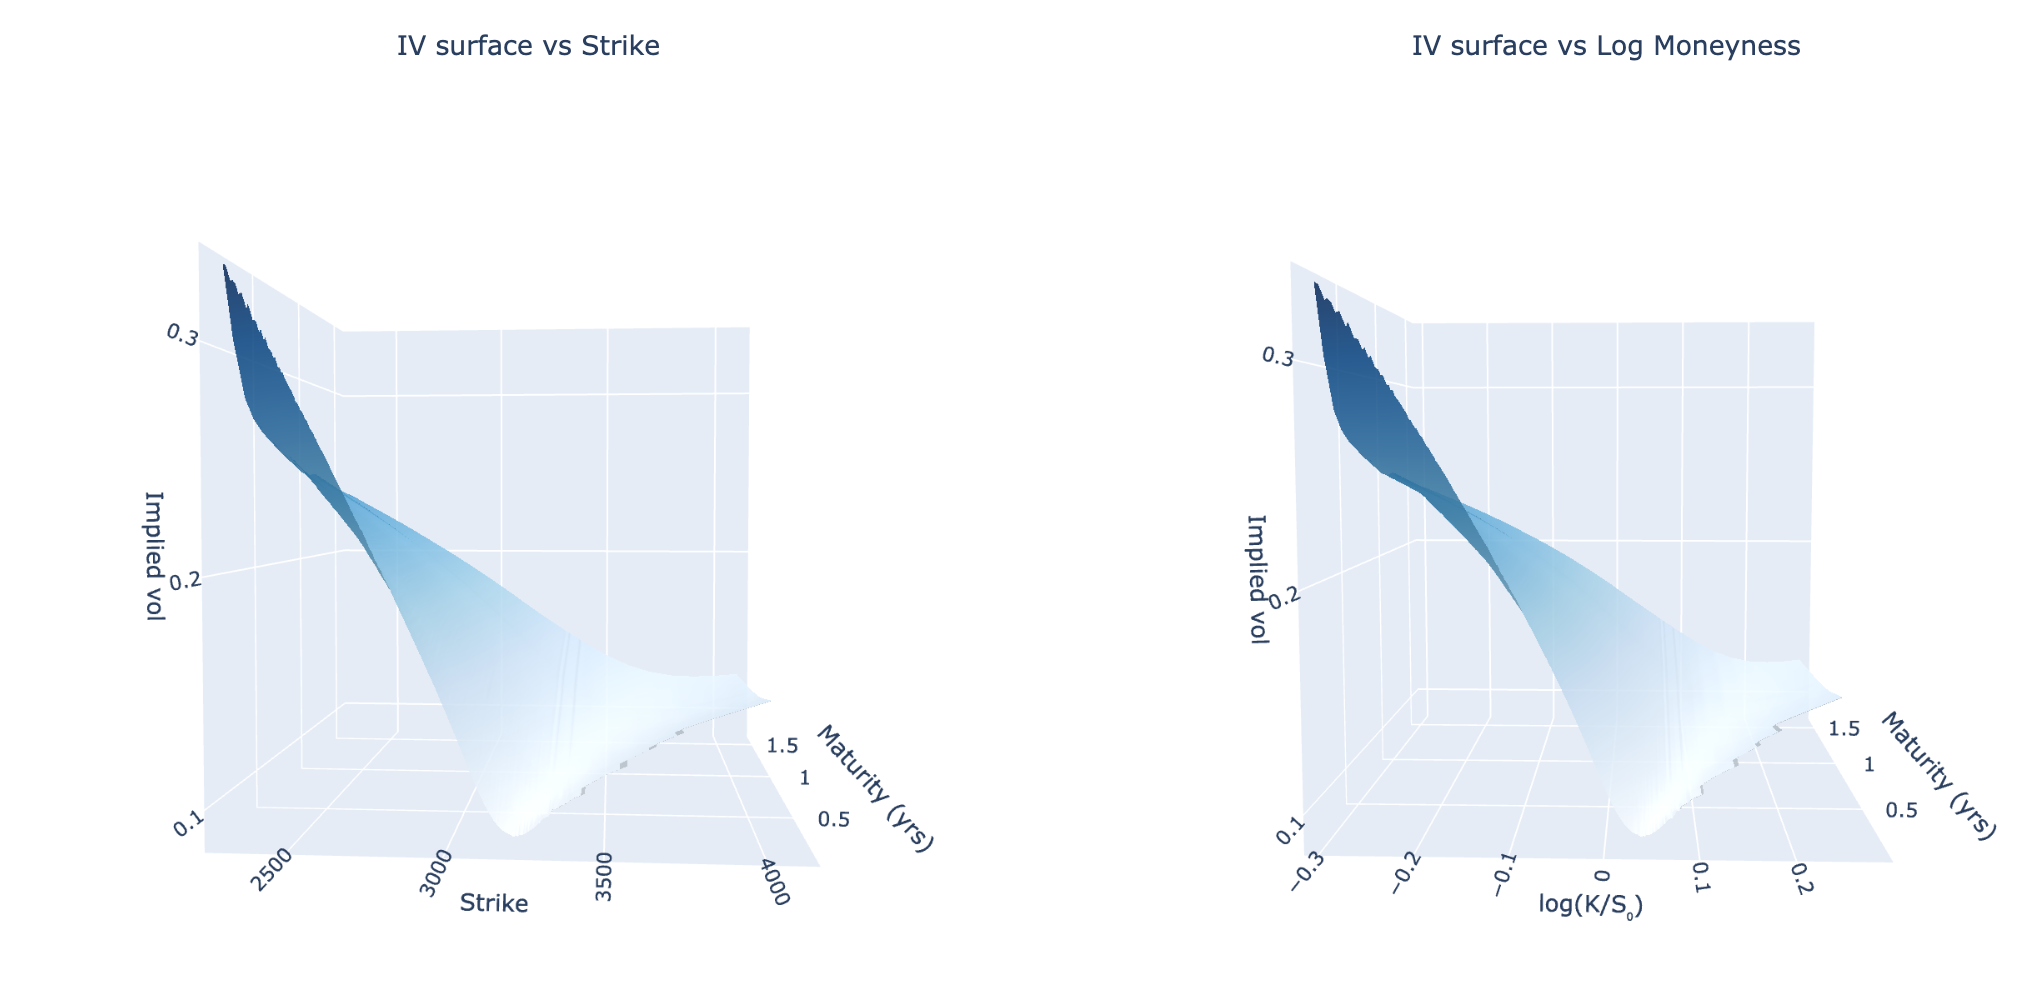
\includegraphics[width=\textwidth]{images/implied_vol_market_only.png}
  \caption{Market implied volatility surface from S\&P 500 options data (13 November 2019, $S_0 = 3094$) after data cleaning, arbitrage filtering, and OTM selection.}
  \label{fig:market-iv-surface}
\end{figure}

\subsection{Numerics}
Before we move on to talking about the calibration of the model to data and the actual fits, we should talk about how it's done. After moving through all the covered data cleaning steps
we want to solve the already discussed minimisation problem. This, however, means calculating a rather large number of integrals depending on the algorithm of choice, for this paper we will be using the ``Trust Region Reflective'' algorithm.
We need to calculate $N$ integrals simply
for evaluating the objective function, to calculate a numerical gradient means multiplying this by some $K > 2$. How hard it will be depends on the choice of quadrature  here the default choice for precision is the Gauss--Kronrod.
However, if speed is a priority, a different choice of quadrature speeds the computation time up significantly. Simply using the trapezoid rule on the interval $[0,400]$ with 4096 splits along with a bit of clever vectorisation in Python
allows us to significantly speed up calculation. To simply forget about anything above 400 seems fine, as we've already shown that the integrand is bounded by an exponential which will already basically have hit 0 at this point.
To showcase the speed increase I've set up a small experiment generating random parameter sets within the bounds:

\begin{center}
\begin{tabular}{lcc}
\textbf{Parameter} & \textbf{Lower} & \textbf{Upper} \\
\hline
$v_0$      & $0.05$ & $0.95$ \\
$\kappa$   & $0.50$ & $5.00$ \\
$\theta$   & $0.05$ & $0.95$ \\
$\sigma$      & $0.50$ & $0.95$ \\
$\rho$     & $-0.95$ & $-0.10$ \\
\end{tabular}
\end{center}

subject to the Feller condition $2\kappa\theta > \sigma^2$,
where we for each parameterset generate Call prices in a grid and try to fit using the different ways of integration. Before we run the experiment we'll add one more thing.
In~\cite{germano2017} they propose a way to calculate analytical gradients within the Heston model. They do this by finding a differentiable expression for the Heston CF and using differentiation under the integral sign to show that
\begin{equation}
\boldsymbol{\nabla} C= \frac{e^{-r\tau}}{\pi}\left[
\int_0^\infty \operatorname{Re}\!\left(\frac{e^{-iu\log\frac{K}{S_0}}}{iu}\,\boldsymbol{\nabla}\psi(u-i,\tau)\right)du
- K\int_0^\infty \operatorname{Re}\!\left(\frac{e^{-iu\log\frac{K}{S_0}}}{iu}\,\boldsymbol{\nabla}\psi(u,\tau)\right)du
\right]
\end{equation}
where $\boldsymbol{\theta}=(v_0,\theta,\rho,\kappa,\sigma)$. I would propose we can, by using their CF expression,
do the same but with the Lewis style formula. It is enough to show that $\frac{d}{d\theta_j}\frac{\Re(\psi(\theta,u,\tau)\cdot e^{-iku})}{\frac{1}{4}+u^2}$ is dominated by some function
$g(u)$ $\forall\theta_j\in\Theta_j$. The Germano et al.\ paper doesn't actually show this directly for their own formula, this also seems a bit out of scope for this paper, so I will simply
implement it and see if it works in the experiment.

\begin{equation}
\boldsymbol{\nabla} C = -\frac{e^{\frac{1}{2}k - rT}}{\pi}
\int_0^\infty \frac{\operatorname{Re}\!\left[e^{-iuk}\,\boldsymbol{\nabla}\psi\!\left(u-\tfrac{i}{2}\right)\right]}{u^2+\tfrac{1}{4}}\,du
\end{equation}
By using this analytical gradient we get to reduce the number of integral calculations when finding the gradient to simply 1 per parameter instead of the at least 2 needed to compute a numerical one.
Remember here that we are borrowing their version~\cite{germano2017} of the Heston CF as well as their partial derivatives. I've implemented this simply to see if it gives us any meaningful speed boost. I implement this
analytical gradient with both quadratures, so we actually get 4 different versions. The experiment will for each round report speed, objective score, and sum of absolute differences in the parameter space
from the solution found in the base case (Gauss--Kronrod) for each method.

\begin{figure}[H]
  \centering
  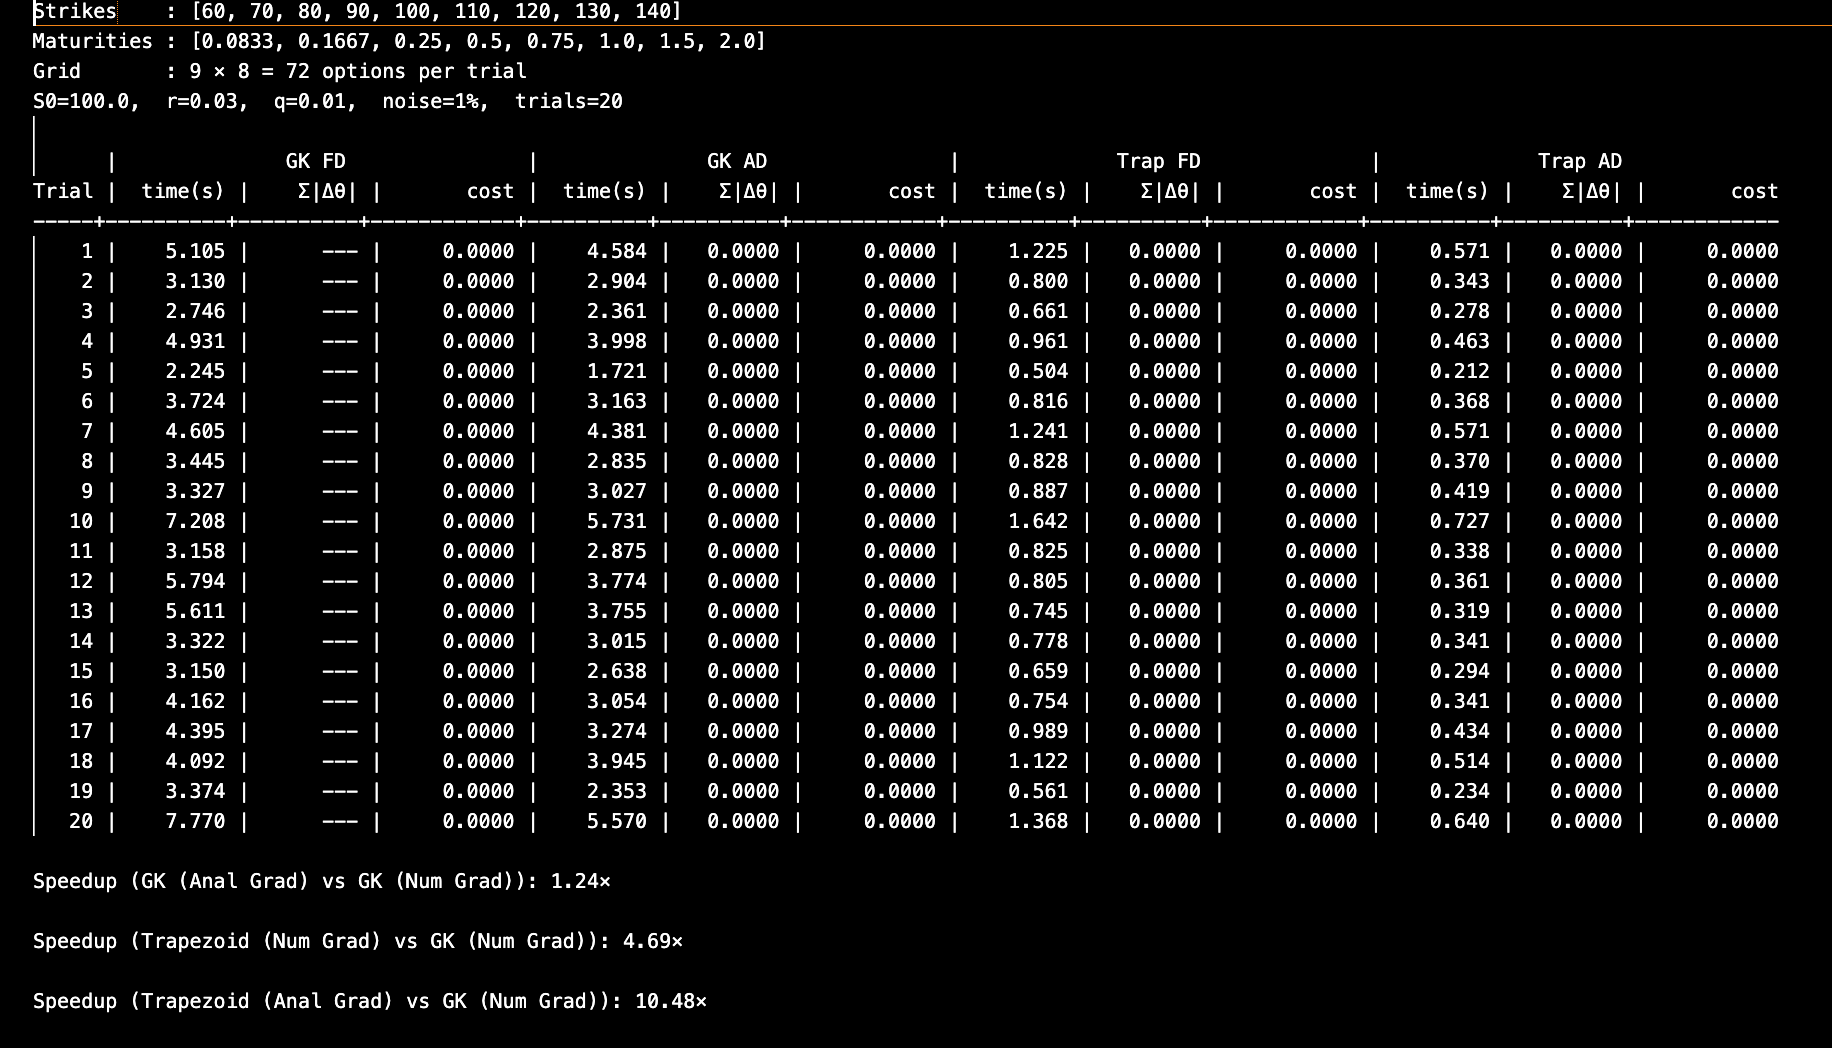
\includegraphics[width=0.9\textwidth]{images/calibration_speed_experiment.png}
  \caption{Calibration speed experiment: wait time and $\sum|\Delta\theta|$ relative to the GK baseline across 20 random Heston parameter draws satisfying the Feller condition. Code for replication can be found in the repo. We see convergence towards the true solution for all the methods, making time the only meaningfull measurement.}
  \label{fig:calibration-speed}
\end{figure}
From the experiment we see that the calibration for all 4 implementations seems to reach the same true minimum, or at least very close to it, and that
especially using the Trapezoid approach over the GK seems to speed us up quite a bit, giving us a 4.69x speed increase. For the GK we get an increase of 25\% from using the analytical gradient, which is of course still
a nice improvement yet less than I expected. Also way less than the 2x improvement we get when going from (Trapezoid -- num.\ diff.) $\rightarrow$ (Trapezoid -- anal.\ diff.), giving us a $\approx$10x speed-up in total.
Some of this improvement will most certainly be due to a better implementation of one or the other. Cutting the calibration to a tenth is still quite nice I think, especially in a situation where where speed matters more, 
imagine a situation where we try to keep a volatility surface generated by the live orderbook wanting to update it as often and quickly as possible. Well, anyway, for this project
speed is a non-issue, meaning we might as well take the slow approach that we know works. Going forward we'll simply use the GK approach with the numerical gradient, using the original Heston CF accounting for the LHT\cite{albrecher2007}.



\subsection{The calibration}
It's now time to calibrate to market data. We run our calibration with the initial guess
$$\omega_0 = (v_0,\kappa,\theta,\sigma,\rho) = (0.04,\ 2.0,\ 0.04,\ 0.4,\ -0.7)$$
once for each weighting getting parameter sets

\begin{center}
\begin{tabular}{lrrrrr}
\textbf{Weighting} & $v_0$ & $\kappa$ & $\theta$ & $\sigma$ & $\rho$ \\
\hline
Unweighted         & 0.0148 & 2.7212 & 0.0495 & 0.8778 & $-0.8290$ \\
Relative (\% error) & 0.0161 & 1.9856 & 0.0625 & 1.0506 & $-0.7648$ \\
\end{tabular}
\end{center}
Looking at the fits it's not hard to notice that they both violate the Feller condition. This however is not an uncommon occurrence when calibrating the Heston model,
and isn't a problem as it doesn't actually invalidate anything in the derivations done above.
Let's see how the implied volatility surfaces generated by these fits look compared to the market. The following surfaces are generated in the repository\cite{github_repo} and additional pictures may be found in the appendix.

\subsubsection{unweighted}

\begin{figure}[H]
  \centering
  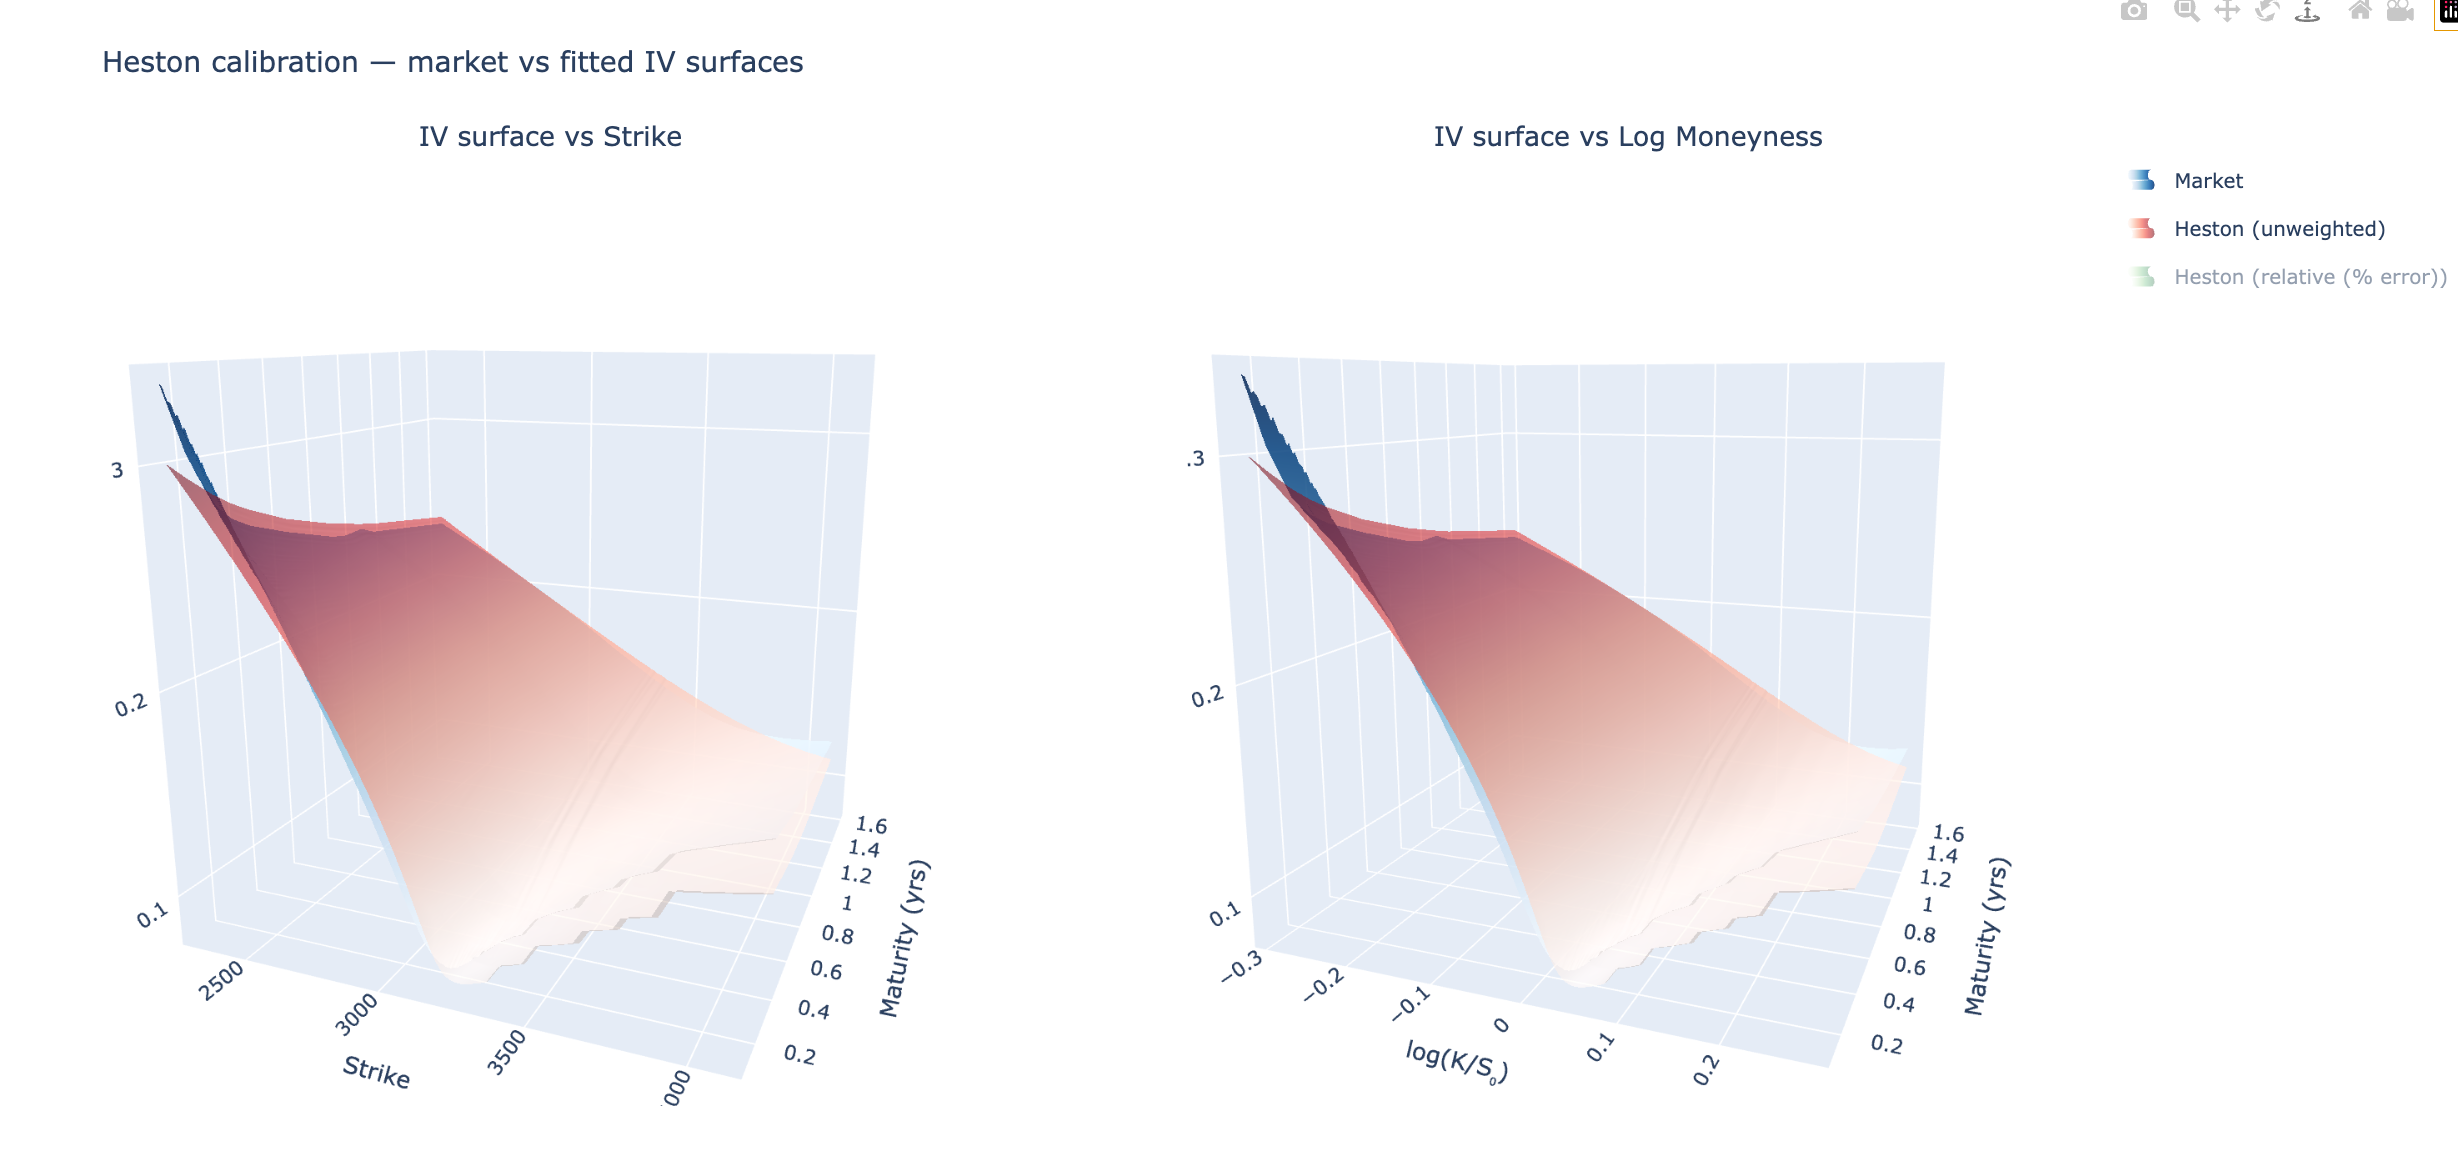
\includegraphics[width=\textwidth]{images/unweighted.png}
  \caption{Heston model fitted IV surface (unweighted calibration) vs.\ market implied volatility surface, S\&P 500 options (13 November 2019, $S_0 = 3094$).}
  \label{fig:iv-fit-unweighted}
\end{figure}

The fit seems to capture the overall shape of the surface quite well, especially on the ITM call side, while pricing OTM calls lower than the market.
This preference to fit the more expensive calls better is however something we expected and is simply a consequence of the choice of objective function.
However, on the very short maturities and low strikes we see that the market trades way higher than the model expects, indicating a higher demand for
deep ITM calls/far OTM puts than the model expects. When going further out on the curve we however see that the surfaces come closer and closer, giving
us a quite good fit on the longer maturity options (1--2 years).


\subsubsection{Relative error}

\begin{figure}[H]
  \centering
  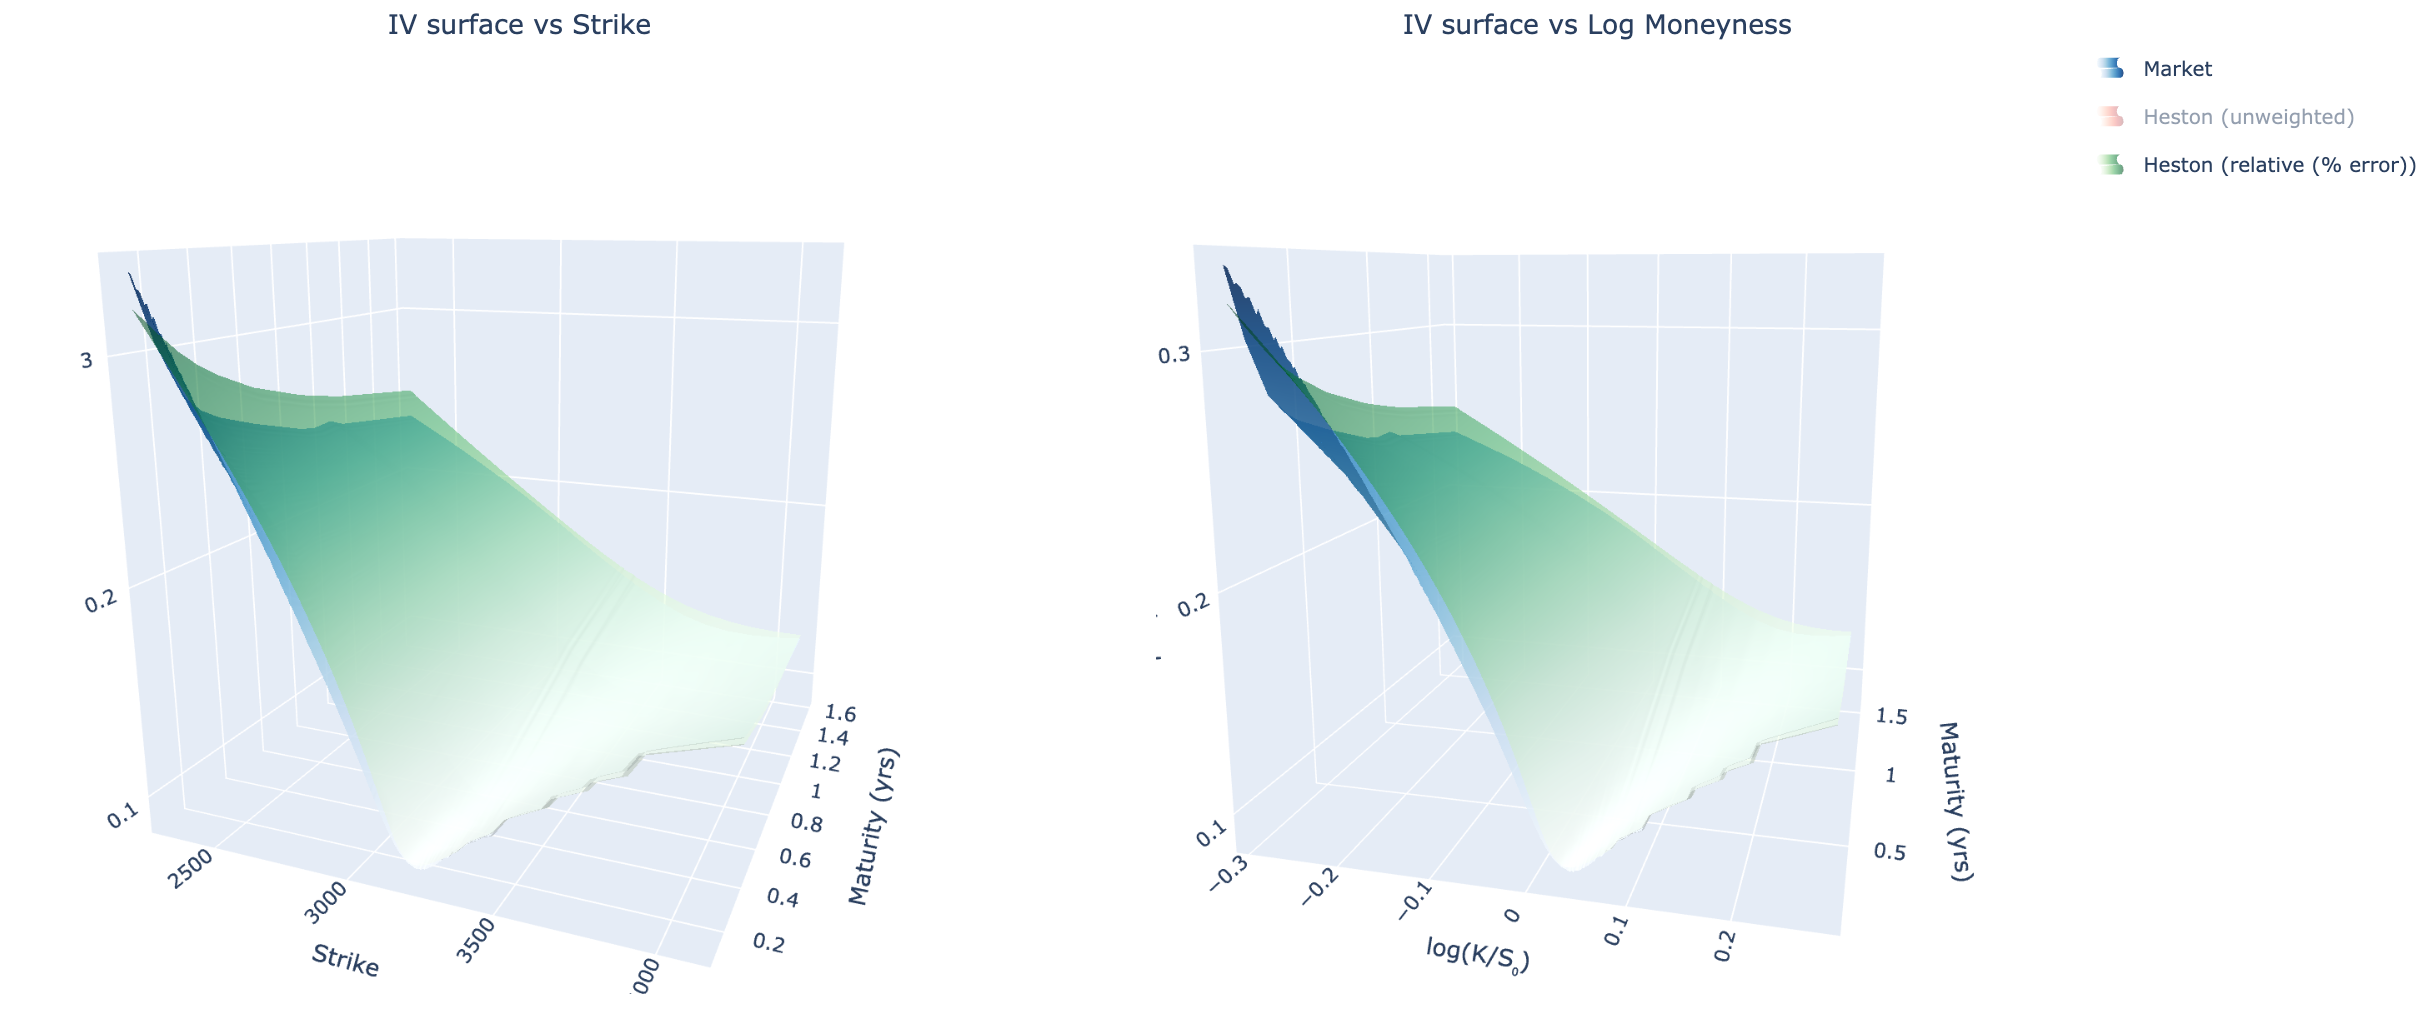
\includegraphics[width=\textwidth]{images/relative.png}
  \caption{Heston model fitted IV surface (relative error weighting) vs.\ market implied volatility surface, S\&P 500 options (13 November 2019, $S_0 = 3094$).}
  \label{fig:iv-fit-relative}
\end{figure}
Again the overall shape is quite good. However, where we before had fitted the ITM calls better, this time we are fitting the OTM side much better. We also see that we price the very short maturities quite well.
This however costs precision on the ITM call side, on longer maturities we are quite far off and never really seem to recover. So the short maturity and OTM sides are priced better. Well, these are for the most
part going to be the cheaper options where a small price error will mean a relatively big gain in the objective function.



To fit the implied volatility surface better we would probably need to switch objective functions into something penalizing errors in implied volatility directly like:
$$\sum_i w_i(\sigma_i^M-\sigma_i^{model})^2$$
this however would mean a worse fit on price, at least in the sum of squares sense, but is still the approach preferred by practitioners\footnote{I asked the options trader on the desk I work on.}.
\sectionwithtoclink{Conclusion}

This paper has covered the theory and practical implementation of the Heston stochastic volatility model from first principles through to calibration on real market data.

We began by deriving the Fourier-based pricing framework by Lewis~\cite{lewis2001}, showing how the covered-call can be priced via a half-line integral formula once the characteristic function of the log asset price is
known and behaves well enough, and how that translates to a call/put price. Once that was established we spent a lot of energy deriving the Heston model CF from the bottom up and arguing that it satisfies the sufficient conditions to
use the Lewis style formula we derived, leaving as few gaps as possible.

On the more practical side we spent some time discussing data handling steps and how differing approaches to the objective function might change the calibration in the end. We then took a small detour to discuss the actual implementation of the pricing engine, from the quadrature choice to mentioning
a way of computing an analytical gradient which might work, and then ran a small experiment comparing these different implementations. This experiment suggests that we are able to reduce the calibration time quite a bit, by going from a Gauss--Kronrod quadrature to a simple calculation using the trapezoid rule,
and by implementing the analytical gradient discussed in~\cite{germano2017}. This isn't necessary for this project at all as we might as well take the more precise approach when time is no issue, but if one considered a
more live version of this pricing engine taking the live order book instead of just a stale day from 2019, one could definitely see the benefit.

We then calibrated the model to closing data from 13/11/2019 with two different weighting schemes. We found that ``no-weighting'' fitted very well to more expensive ITM calls at the expense of cheaper ones, while the ``relative-error''
weighting prioritises the cheaper ITM and short-duration options. Both calibrations, however, captured the overall shape of the volatility surface quite well.

Natural ways to capture more of the shape of the volatility surface would of course be to add more complexity. This could include jumps, an additional vol process, or making the vol-of-vol process stochastic too, or as discussed simply targeting the implied volatilities directly.
 




\sectionwithtoclink{Appendix}
\renewcommand{\thefigure}{A.\arabic{figure}}
\setcounter{figure}{0}
\subsection{Generalised Fourier Inversion}
\label{app:gen_fourier}

For $f:\mathbb{R}\to\mathbb{C}$ and $\alpha\in\mathbb{R}$, define
\begin{equation}
    \hat{f}(u + i\alpha) = \int_{-\infty}^{\infty} e^{i(u+i\alpha)x} f(x)\, dx.
\end{equation}
Suppose that
\begin{equation}
    e^{-\alpha x}f(x) \in L^1(\mathbb{R})
    \qquad \text{and} \qquad
    \hat{f}(\,\cdot + i\alpha) \in L^1(\mathbb{R}).
\end{equation}
Then
\begin{equation}
    f(x) = \frac{1}{2\pi}
    \int_{-\infty}^{\infty}
    e^{-i(u+i\alpha)x}\,\hat{f}(u+i\alpha)\,du \qquad \text{a.e.}
\end{equation}

\begin{definition}[Strip of Regularity]
    Let $f : \mathbb{R} \to \mathbb{C}$. The \emph{strip of regularity} of $f$ is
    \begin{equation}
        S_f := \left\{ z \in \mathbb{C} : e^{izx}f(x) \in L^1(\mathbb{R}) \right\}
        = \left\{ u + i\alpha : e^{-\alpha x}f(x) \in L^1(\mathbb{R}) \right\}.
    \end{equation}
    This is a horizontal strip $S_f = \{ z : \mathrm{Im}\, z \in (a, b) \}$ for
    some $-\infty \leq a < b \leq \infty$, on which the generalised Fourier
    transform
    \begin{equation}
        \hat{f}(z) := \int_{-\infty}^{\infty} e^{izx} f(x)\, dx
    \end{equation}
    is well-defined as we don't have divergence issues
\end{definition}

\subsection{stochastic calculus}
The results in this section follow~\cite{baudouin2019}.
consider the filtered probability space $(\Omega,\mathcal{F},\mathcal{F}_{t\geq0},\mathbb{P})$ on this define a n-dimensional standard brownian motion
$(B_t)_{t\geq0}$ and functions $b,\sigma:\mathbb{R}^n\rightarrow \mathbb{R}^n$
under regularity conditions that the heston model satisfies we have:

consider the SDE
\begin{align}
dX_t^x &=b(X_t^x) dt + \sigma(X_t^x)dB_t
\end{align}
look at $B=\{f\in C^2:f\quad has\,\, polynomial\,\, growth\}$ we then define $L:B\rightarrow C$
\begin{align}
L f(x)
=
\sum_{i=1}^n b_i(x)\,\frac{\partial f}{\partial x_i}(x)
+
\frac{1}{2}
\sum_{i,j=1}^n a_{ij}(x)\,\frac{\partial^2 f}{\partial x_i \partial x_j}(x).
\end{align}
where $a(x)=\sigma(x)\sigma(x)^*$

\subsubsection{ito's lemma}

\begin{theorem}[Multidimensional It\^{o}'s Lemma]
Let $X_t = (X_t^1,\ldots,X_t^n)^T$ be the solution to the multivariate SDE
\begin{equation}
dX_t = b(X_t)\,dt + \sigma(X_t)\,dW_t,
\end{equation}
where $b:\mathbb{R}^n\to\mathbb{R}^n$, $\sigma:\mathbb{R}^n\to\mathbb{R}^{n\times m}$,
and $W_t$ is an $m$-dimensional standard Brownian motion.
Let $f\in C^{1,2}([0,T]\times\mathbb{R}^n)$. Then
\begin{equation}
df(t,X_t)
=\frac{\partial f}{\partial t}(t,X_t)\,dt
+\sum_{i=1}^{n}\frac{\partial f}{\partial x_i}(t,X_t)\,dX_t^i
+\frac{1}{2}\sum_{i,j=1}^{n}a_{ij}(X_t)\,\frac{\partial^2 f}{\partial x_i\,\partial x_j}(t,X_t)\,dt,
\end{equation}


\end{theorem}
\subsubsection{the feyman kac formula}

\begin{theorem}
Let \( f : \mathbb{R}^n \to \mathbb{R} \) be a Borel function with polynomial growth.

Let \( u : [0, +\infty) \times \mathbb{R}^n \to \mathbb{R} \) be a solution to:
\begin{align}
\frac{\partial u}{\partial t}(t, x) = Lu(t, x)
\end{align}
where t is taken as a constant when applying the operator L\\
with the initial condition
\begin{align}
u(0, x) = f(x).
\end{align}

If there exists a locally integrable function \( C \) and \( p \geq 0 \), such that for every \( t \geq 0 \) and \( x \in \mathbb{R}^n \),
\begin{align}
\|\nabla u(t, x)\| \leq C(t)\left(1 + \|x\|^p\right),
\end{align}
then
\begin{align}
u(t, x) = \mathbb{E}[f(X_t^x)].
\end{align}
\end{theorem}

notes:
\begin{itemize}
\item[$\bullet$] f has polinomial growth $\Leftrightarrow \exists c>0,p\geq 0:|f(x)|\leq c(1+\vert x \vert^p)\forall x\in\mathbb{R}$
\item[$\bullet$] C locally integrable $\Leftrightarrow \int_K C \,d\mu<\infty \text{ for } K \subseteq \mathbb{R} \text{ Compact}$
\item[$\bullet$] the result works in the more general case with $u(t-s)=\mathbb{E}[f(X_t^x)|\mathcal{F}_s]$
\end{itemize}


\subsection{derivations}

\subsubsection{$L^1$ bound for $\psi(\cdot-i/2)$}
\label{app:l1bound}
\begin{align}
a &= \kappa - \frac{\rho\sigma}{2}, \\
c &= \frac{\sigma\sqrt{1-\rho^2}}{2}.
\end{align}


\begin{equation}
\gamma = \frac{\sqrt{1-\rho^2}}{2\sigma}\bigl(\kappa\theta T + v_0\bigr).
\end{equation}

$U = \max(U_1, U_2, U_3)$ with
\begin{align}
U_1 &= \sqrt{\frac{2(a^2+\tfrac{\sigma^2}{4}+1)+\sigma^2(1-\rho^2)}{\sigma^2(1-\rho^2)}},\\
U_2 &= \frac{4|a|}{\sigma\sqrt{1-\rho^2}},\\
U_3 &= \frac{1}{cT}.
\end{align}
$K = \exp(\log K)$ where
\begin{equation}
\log K = \frac{\kappa^2\theta T}{\sigma^2}
        +\left|\frac{\kappa\theta\rho T}{2\sigma}\right|
        +\left|\frac{(r-q)T}{2}\right|
        +\frac{2\kappa\theta}{\sigma^2}\left|\log\frac{\sqrt{1+\rho^2}}{4}\right|
        +\frac{v_0|a|}{\sigma^2}
        +\gamma U.
\end{equation}






\subsection{Figures}

\begin{figure}[H]
  \centering
  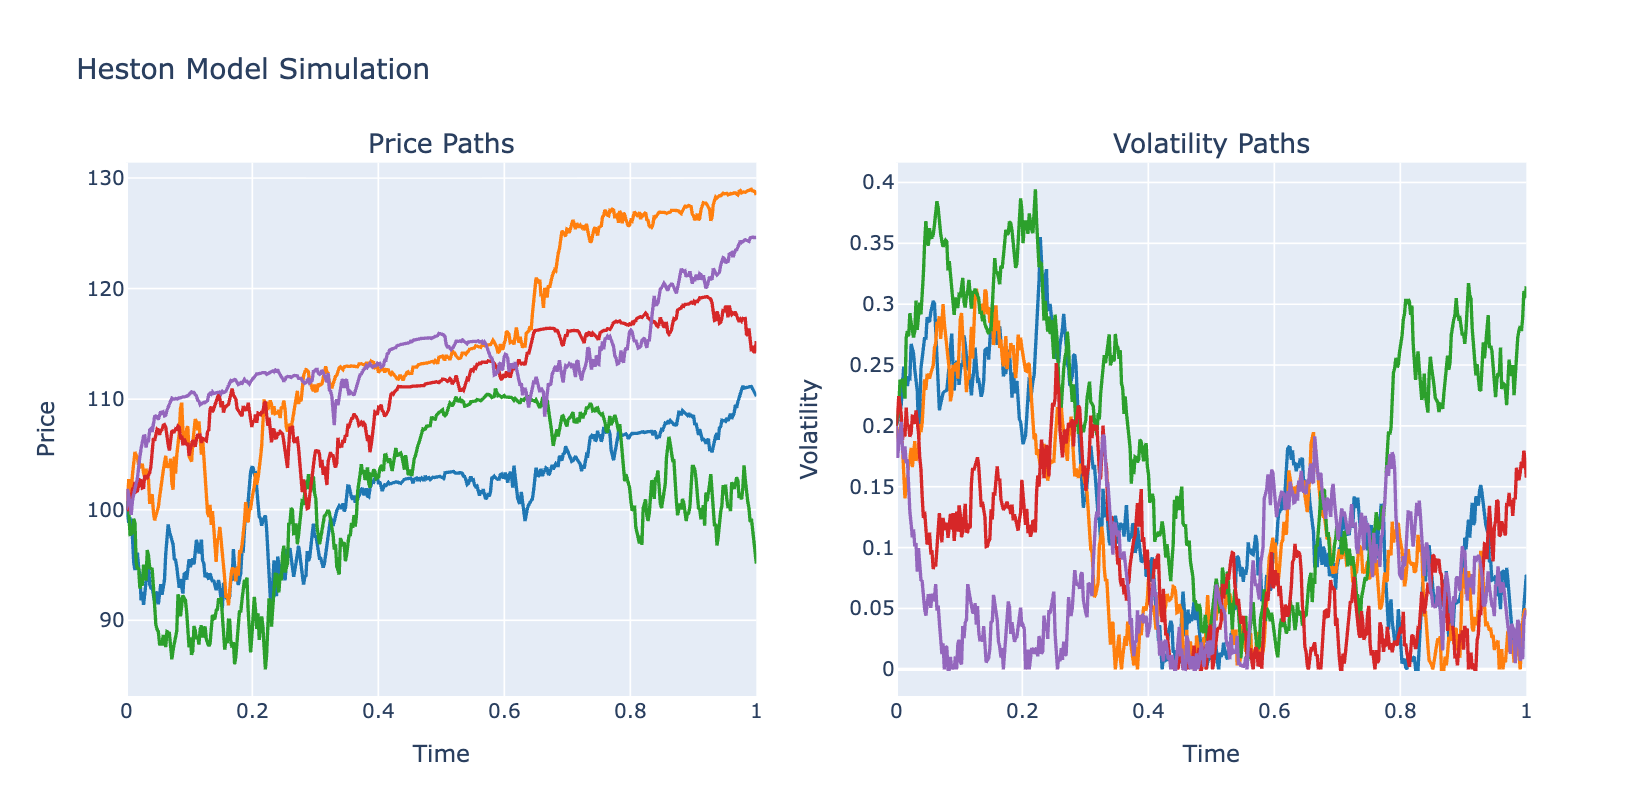
\includegraphics[width=\textwidth]{images/model_simulation.png}
  \caption{Simulated Heston model paths for the asset price and variance process using a Milstein-corrected Euler scheme ($S_0=100$, $v_0=0.04$, $\kappa=2.0$, $\theta=0.04$, $\sigma=0.6$, $\rho=-0.7$, $r=0.05$, $q=0.02$, $T=1$, $N=512$).}
  \label{fig:heston-simulation-app}
\end{figure}

\begin{figure}[H]
  \centering
  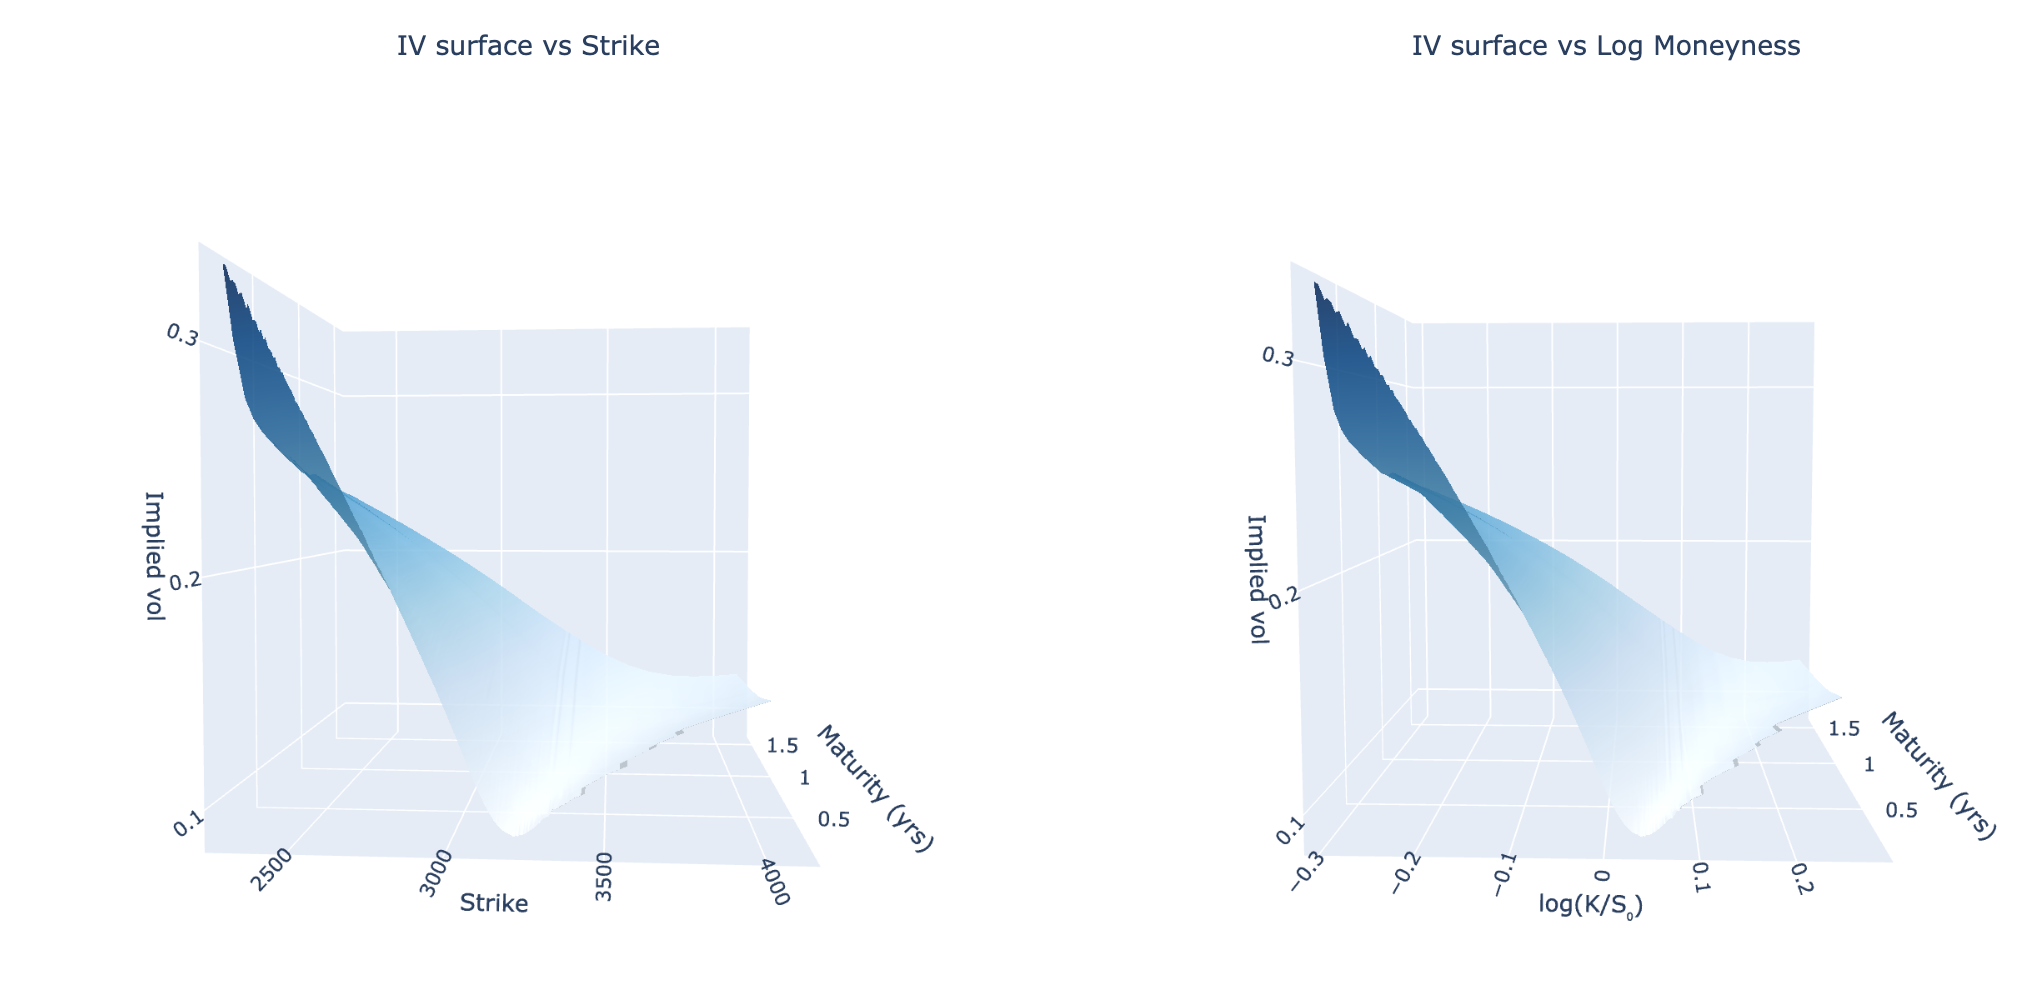
\includegraphics[width=\textwidth]{images/implied_vol_market_only.png}
  \caption{Market implied volatility surface from S\&P 500 options data (13 November 2019, $S_0 = 3094$) after data cleaning and arbitrage filtering, plotted against strike and log-moneyness.}
  \label{fig:market-iv-surface-app}
\end{figure}

\begin{figure}[H]
  \centering
  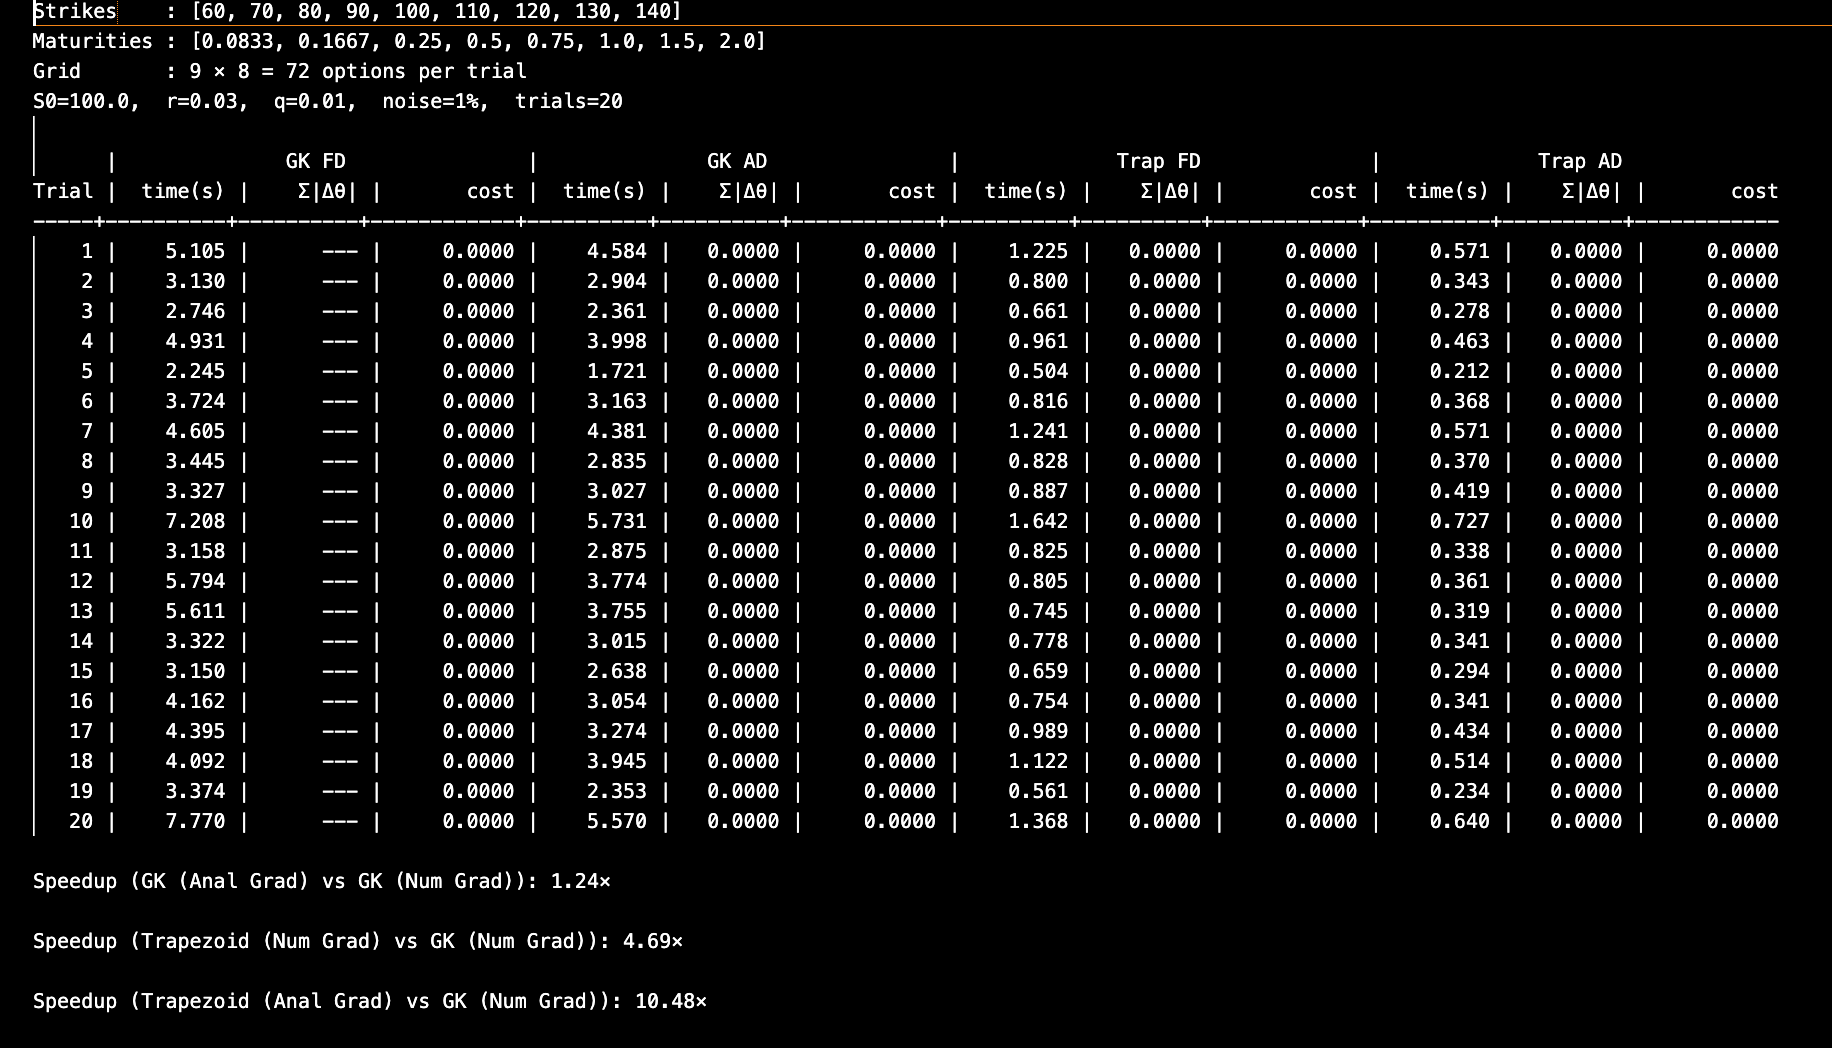
\includegraphics[width=\textwidth]{images/calibration_speed_experiment.png}
  \caption{Calibration speed experiment: wall time and $\sum|\Delta\sigma|$ relative to the GK baseline across 20 random Heston parameter draws satisfying the Feller condition.}
  \label{fig:calibration-speed-app}
\end{figure}

\begin{figure}[H]
  \centering
  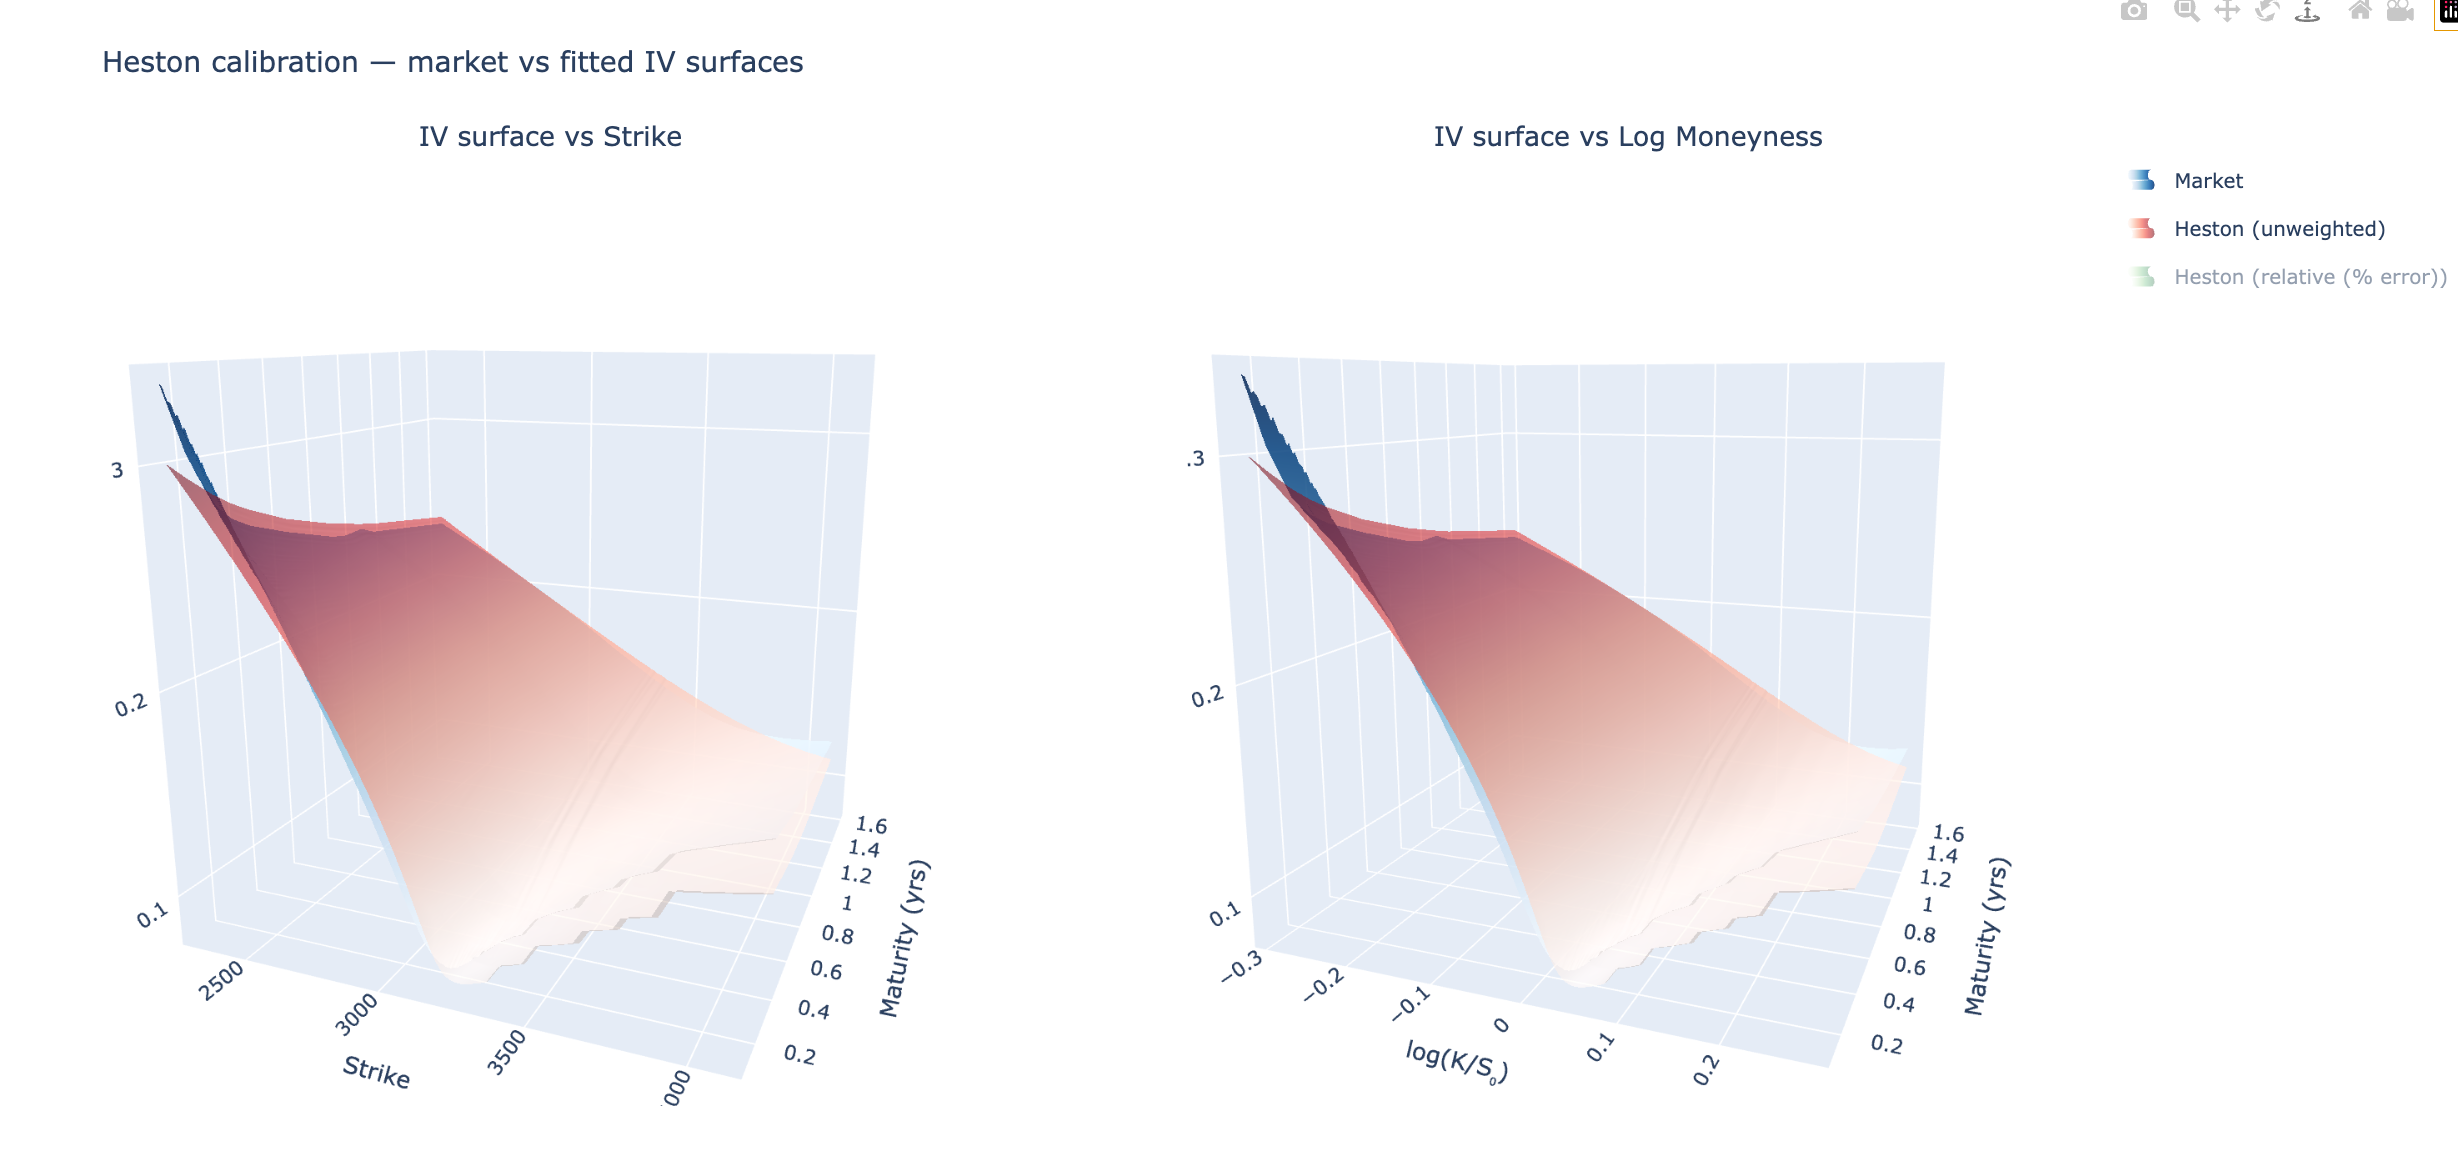
\includegraphics[width=\textwidth]{images/unweighted.png}
  \caption{Heston model fitted IV surface (unweighted calibration) vs.\ market implied volatility surface, S\&P 500 options (13 November 2019, $S_0 = 3094$).}
  \label{fig:iv-fit-unweighted-app}
\end{figure}

\begin{figure}[H]
  \centering
  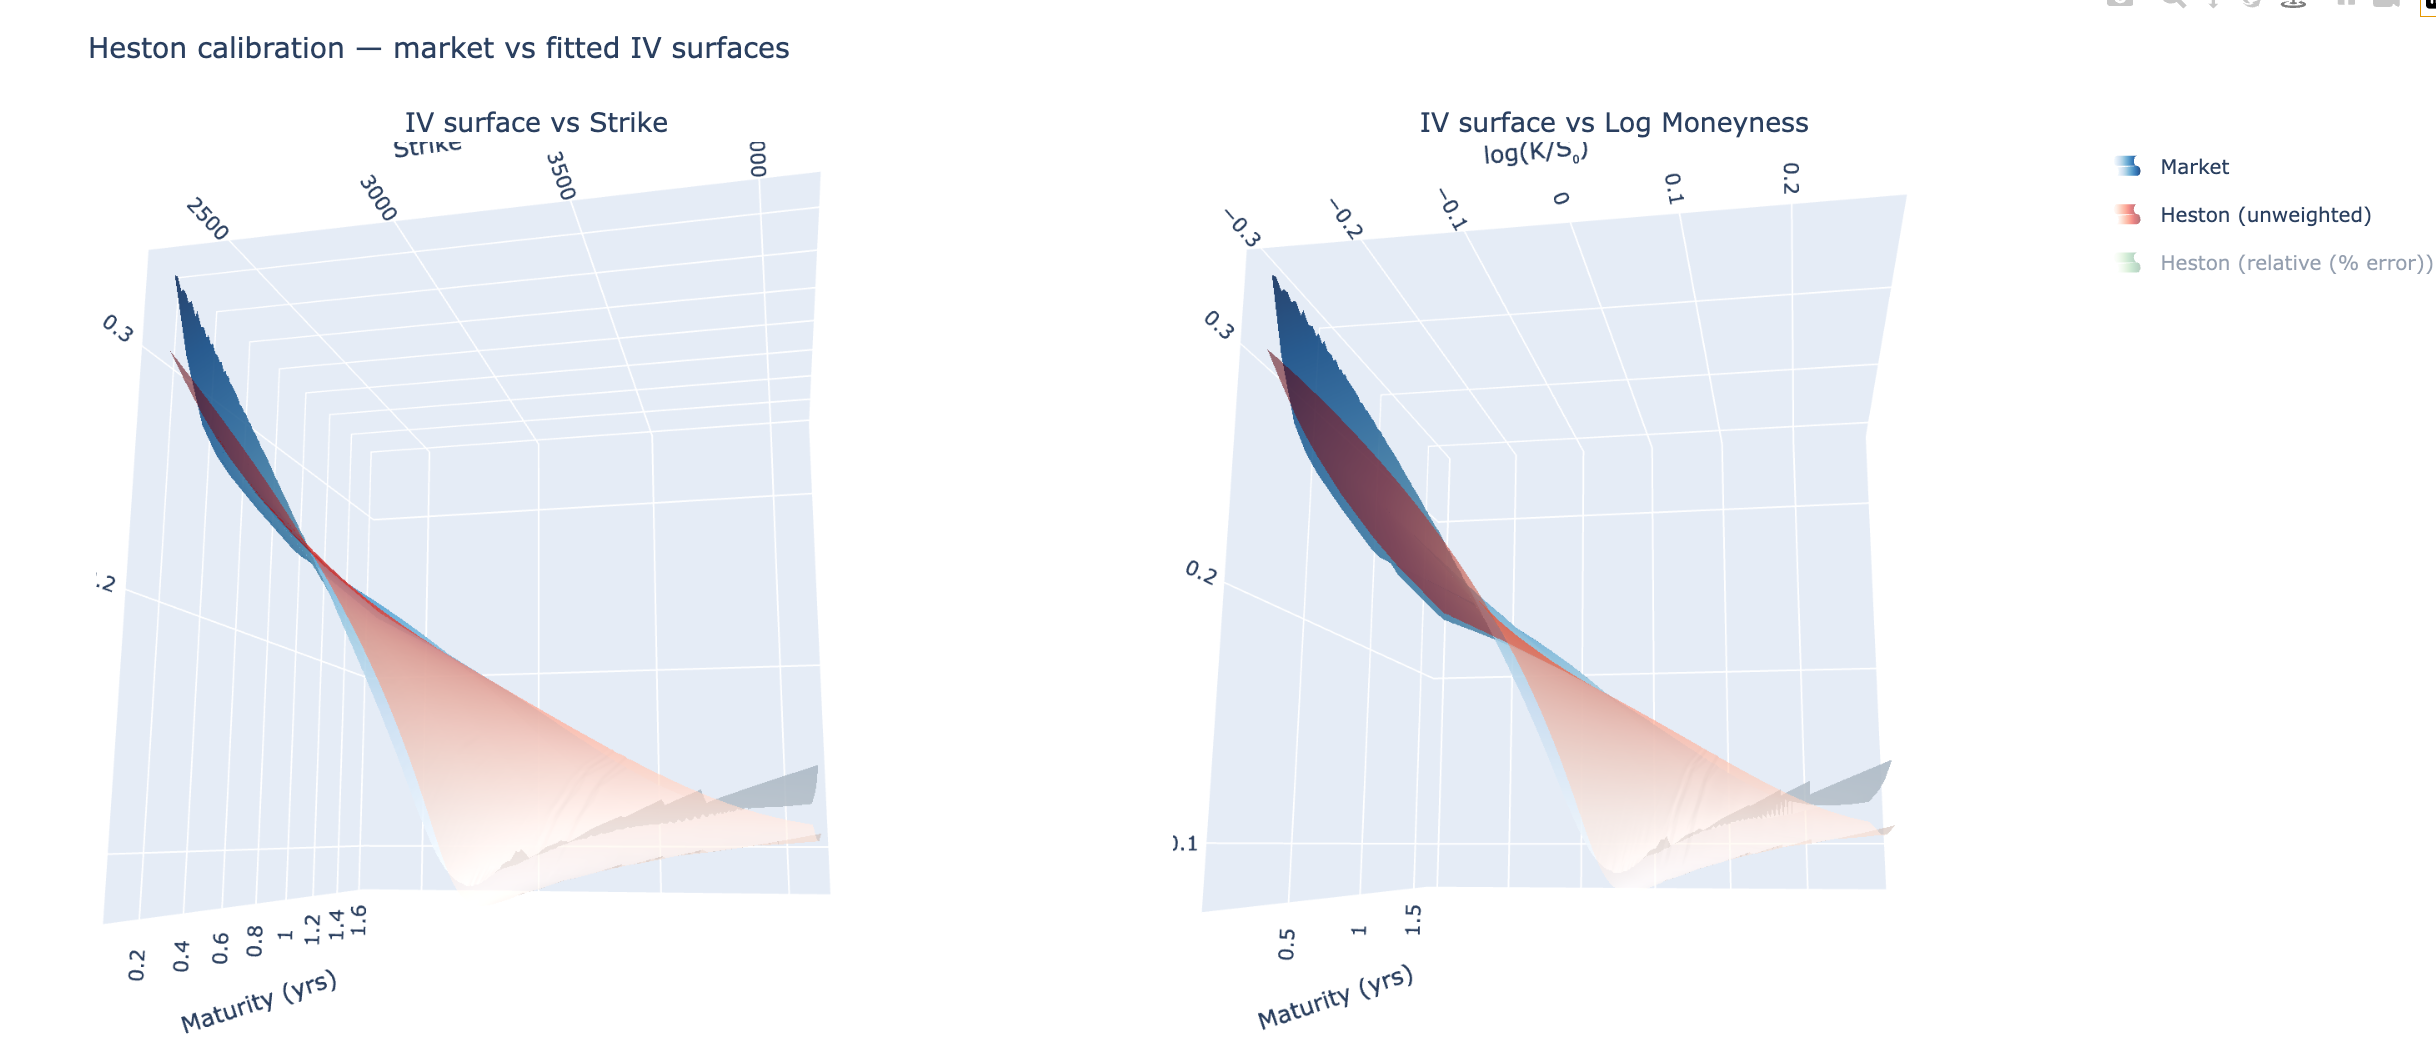
\includegraphics[width=\textwidth]{images/unweighted2.png}
  \caption{Alternative viewing angle of the Heston fitted IV surface (unweighted calibration) vs.\ market implied volatility surface, S\&P 500 options (13 November 2019, $S_0 = 3094$).}
  \label{fig:iv-fit-unweighted2}
\end{figure}

\begin{figure}[H]
  \centering
  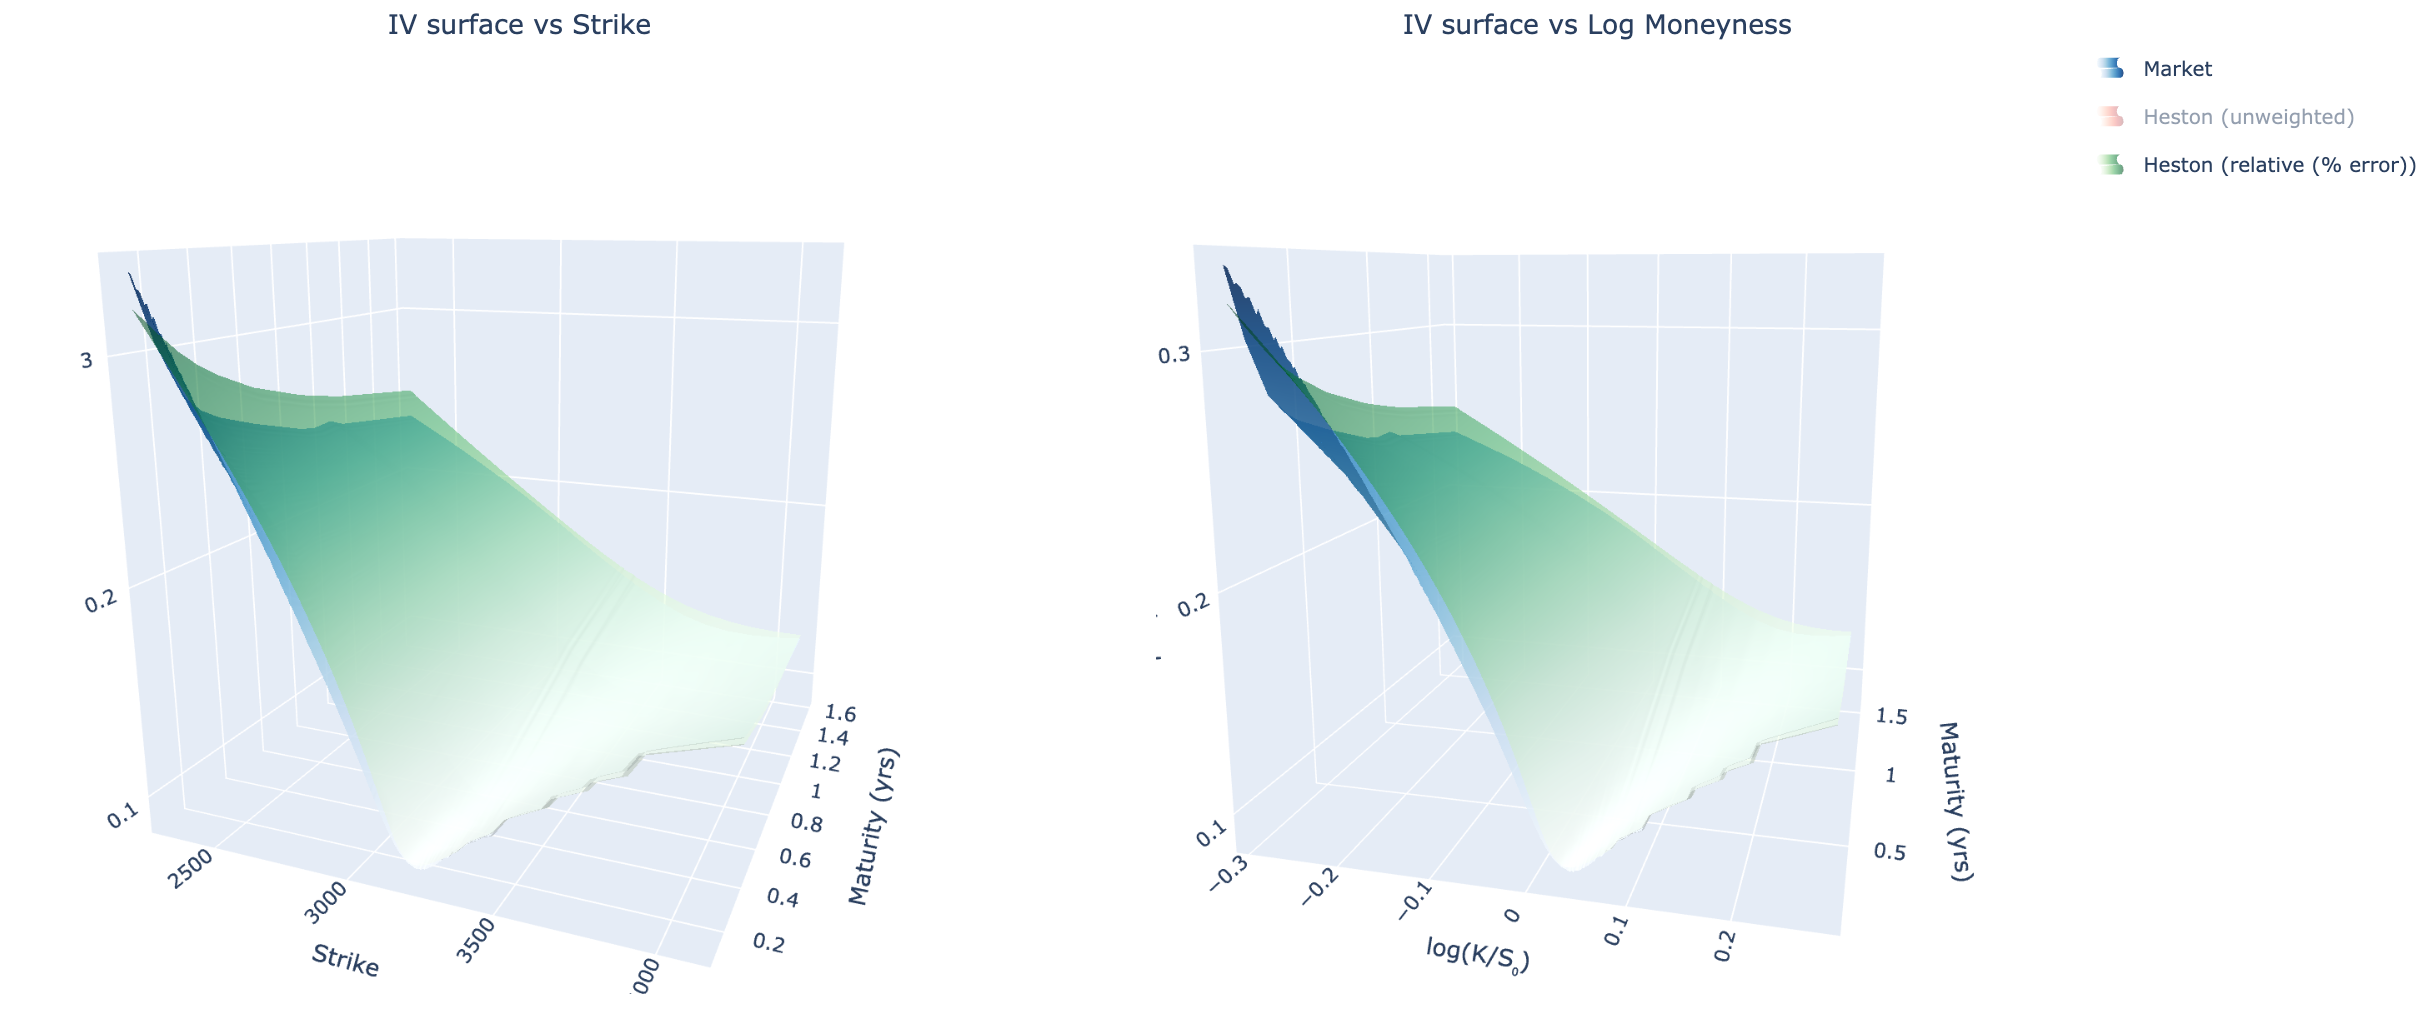
\includegraphics[width=\textwidth]{images/relative.png}
  \caption{Heston model fitted IV surface (relative error weighting) vs.\ market implied volatility surface, S\&P 500 options (13 November 2019, $S_0 = 3094$).}
  \label{fig:iv-fit-relative-app}
\end{figure}

\begin{figure}[H]
  \centering
  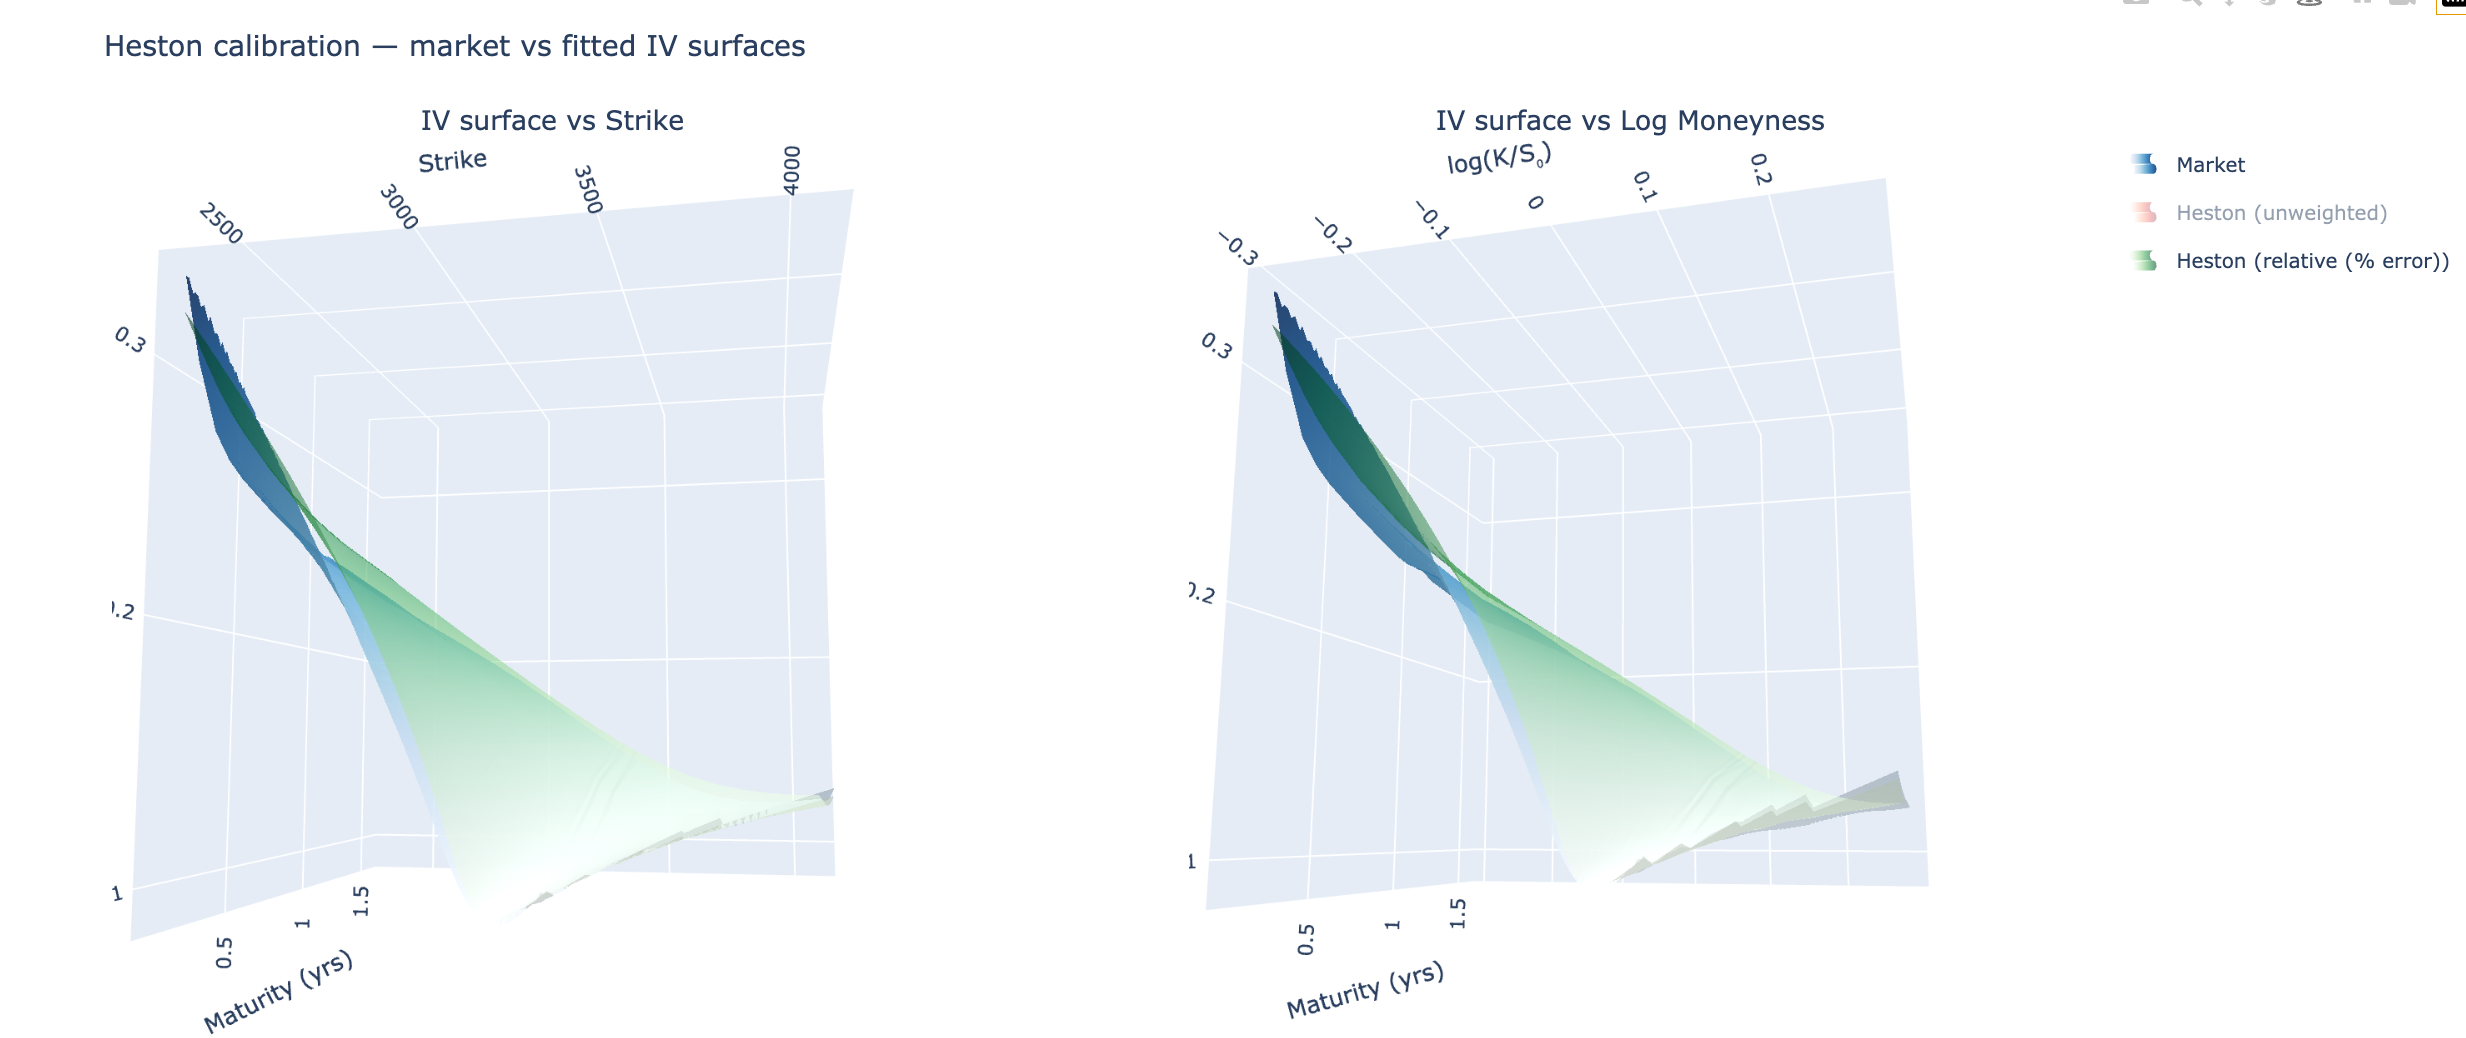
\includegraphics[width=\textwidth]{images/relative2.png}
  \caption{Alternative viewing angle of the Heston fitted IV surface (relative error weighting) vs.\ market implied volatility surface, S\&P 500 options (13 November 2019, $S_0 = 3094$).}
  \label{fig:iv-fit-relative2}
\end{figure}

\subsection{code}
The code generated making this project can be found in the github repo~\cite{github_repo}, in there is a read me explaining the
code structure, and how to run it replicating everything with seeding 


\bibliographystyle{unsrt}
\bibliography{references}

\end{document}
